\documentclass[10pt]{article}\usepackage[]{graphicx}\usepackage[]{xcolor}
% maxwidth is the original width if it is less than linewidth
% otherwise use linewidth (to make sure the graphics do not exceed the margin)
\makeatletter
\def\maxwidth{ %
  \ifdim\Gin@nat@width>\linewidth
    \linewidth
  \else
    \Gin@nat@width
  \fi
}
\makeatother

\definecolor{fgcolor}{rgb}{0.345, 0.345, 0.345}
\newcommand{\hlnum}[1]{\textcolor[rgb]{0.686,0.059,0.569}{#1}}%
\newcommand{\hlsng}[1]{\textcolor[rgb]{0.192,0.494,0.8}{#1}}%
\newcommand{\hlcom}[1]{\textcolor[rgb]{0.678,0.584,0.686}{\textit{#1}}}%
\newcommand{\hlopt}[1]{\textcolor[rgb]{0,0,0}{#1}}%
\newcommand{\hldef}[1]{\textcolor[rgb]{0.345,0.345,0.345}{#1}}%
\newcommand{\hlkwa}[1]{\textcolor[rgb]{0.161,0.373,0.58}{\textbf{#1}}}%
\newcommand{\hlkwb}[1]{\textcolor[rgb]{0.69,0.353,0.396}{#1}}%
\newcommand{\hlkwc}[1]{\textcolor[rgb]{0.333,0.667,0.333}{#1}}%
\newcommand{\hlkwd}[1]{\textcolor[rgb]{0.737,0.353,0.396}{\textbf{#1}}}%
\let\hlipl\hlkwb

\usepackage{framed}
\makeatletter
\newenvironment{kframe}{%
 \def\at@end@of@kframe{}%
 \ifinner\ifhmode%
  \def\at@end@of@kframe{\end{minipage}}%
  \begin{minipage}{\columnwidth}%
 \fi\fi%
 \def\FrameCommand##1{\hskip\@totalleftmargin \hskip-\fboxsep
 \colorbox{shadecolor}{##1}\hskip-\fboxsep
     % There is no \\@totalrightmargin, so:
     \hskip-\linewidth \hskip-\@totalleftmargin \hskip\columnwidth}%
 \MakeFramed {\advance\hsize-\width
   \@totalleftmargin\z@ \linewidth\hsize
   \@setminipage}}%
 {\par\unskip\endMakeFramed%
 \at@end@of@kframe}
\makeatother

\definecolor{shadecolor}{rgb}{.97, .97, .97}
\definecolor{messagecolor}{rgb}{0, 0, 0}
\definecolor{warningcolor}{rgb}{1, 0, 1}
\definecolor{errorcolor}{rgb}{1, 0, 0}
\newenvironment{knitrout}{}{} % an empty environment to be redefined in TeX

\usepackage{alltt}

\usepackage{times}
\RequirePackage{natbib}
\usepackage[colorlinks=true, citecolor=blue, linkcolor=blue]{hyperref}
\usepackage{amsmath, amssymb, fullpage, amsthm, array, graphicx, asa, url}

\graphicspath{{images/}}

% JASA guideline to have double spaced fonts
\usepackage{setspace}
\doublespacing


\usepackage{color}
\definecolor{mahbub}{rgb}{1.0, 0.6, 0.4}

\newcommand{\hh}[1]{{\color{magenta} #1}}
\newcommand{\dc}[1]{{\color{green} #1}}
\newcommand{\mm}[1]{{\color{mahbub} #1}}
\renewcommand*\familydefault{\sfdefault} % To make font Halvatica, Wiley requirement

\setlength{\oddsidemargin}{0in}
\setlength{\evensidemargin}{0in}
\setlength{\textwidth}{6.5in}
\setlength{\topmargin}{-0.4in}
\setlength{\textheight}{9in}
\evensidemargin 
\oddsidemargin

\pdfminorversion=4 % as instructed by JASA file upload
% NOTE: To produce blinded version, replace "1" with "0" below. 
% Blinded version will also remove acknowledgement at the bottom.
\newcommand{\blindDoc}{1}
\IfFileExists{upquote.sty}{\usepackage{upquote}}{}
\begin{document}

% ===================================================================================
%Article top matter 
%------------------------------------------------------------------------------------

\if1\blindDoc
{
  \title{Effect of Sociological Factors on Visual Statistical Inference}
  \author{{Mahbubul Majumder, Heike Hofmann, Dianne Cook}
\thanks{Mahbubul Majumder is an Associate Professor in the Department of Mathematical and Statistical Sciences, University of Nebraska Omaha, NE 68182 (e-mail: mmajumder@unomaha.edu), Heike Hofmann is Professor in the Department of Statistics, University of Nebraska Lincoln, NE, and  Dianne Cook is Professor in the Department of Econometrics and Business Statistics, Monash University, Australia. This research is supported in part by the National Science Foundation Grant \# DMS 1007697.}}
\date{\vspace{-.5in}}
  \maketitle
} \fi

\if0\blindDoc
{
  \bigskip
  \bigskip
  \bigskip
  \begin{center}
    {\bf \LARGE Human Factors Influencing Visual Statistical Inference}
\end{center}
  \medskip
} \fi


% ===================================================================================
\begin {abstract} 
%------------------------------------------------------------------------------------

Visual statistical inference determines the significance of patterns found in data exploration through graphics. It involves human observers inspecting a lineup of plots, with one real data plot randomly placed among decoys. Each observer's cognitive skills and judiciousness can influence results. The effectiveness of this method, measured by power, depends on combining evaluations from multiple observers. Factors influencing power include observer demographics, visual skills, experience, the sample of null plots, plot position, and signal strength. This paper examines these factors through studies using Amazon's Mechanical Turk, finding individual skills vary but demographics have little impact. Learning increases speed but not accuracy, and plot position doesn’t affect results.

{\bf Keywords: \sf statistical graphics, non-parametric test, cognitive psychology, data visualization, exploratory data analysis, data mining, visual analytics.} 
\end {abstract}

% ===================================================================================
\section{Introduction}  
%------------------------------------------------------------------------------------

%The lineup protocol introduced in \citet{buja:2009} can be used to quantify the significance of graphical findings in the exploratory data analysis process. This methodology is  part of what is called visual statistical inference, which has been developed further  and validated by \citet{majumder:2013} in simulation studies of head to head comparisons with conventional inference. One of their major contributions is to define the power of  visual tests and to provide a method for obtaining the power for a particular lineup. In some scenarios, the power of a visual test  was seen to outperform that of a conventional test.

%In visual inference, the test statistic is a plot of the observed data, called the {\it (actual) data plot}. To create a lineup the data plot is placed randomly in a grid of null plots. Null plots  are rendered from data generated as  specified by a null hypothesis. Often, this null hypothesis assumes independence or no structure in the data. An observer is then asked to evaluate the lineup. If the  actual data plot is detected by the observer, this counts as evidence against the null hypothesis. Based on the number of evaluations by independent observers and the number of times that the data plot is identified, we are  able to evaluate the significance of the graphical relationship in the same way and the same rigor as a conventional hypothesis test. 


The lineup protocol introduced by \citet{buja:2009} quantifies the significance of graphical findings in exploratory data analysis, forming part of visual statistical inference. \citet{majumder:2013} extended and validated this approach through simulation studies, showing that visual inference can sometimes outperform conventional methods. They also defined the power of visual tests and proposed a way to calculate it for a given lineup. In visual inference, the test statistic is a plot of observed data, randomly placed among null plots generated under a null hypothesis, often assuming no structure. Observers evaluate the lineup, and if they consistently identify the data plot, this provides evidence against the null hypothesis, akin to a conventional hypothesis test.


% \begin{figure}[hbtp] 
%    \centering
%    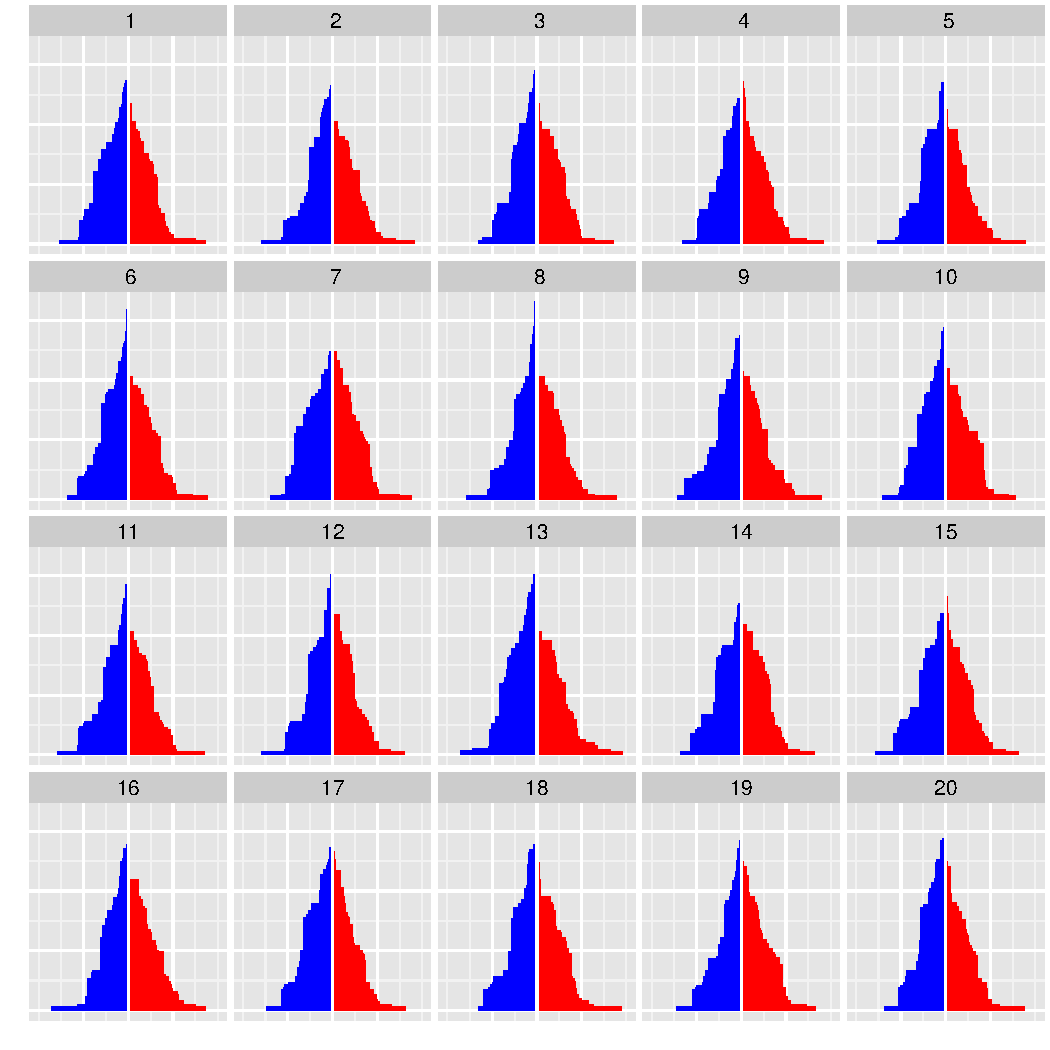
\includegraphics[width=0.99\textwidth]{electoral-5-13.pdf} 
%    \caption{ \label{fig:elect} Which one of the plots, labelled 1 through 20 from top left to bottom right, is the most different from the others?}
% \end{figure}

%Figure~\ref{fig:elect} displays an example lineup, one of the plots is based on the observed data, while the remaining 19 plots show  data generated from a null model. Which one of the 20 plots is the most different from the others? 
%When asked this question, 12 out of 72 observers picked the  data plot located in panel number $4^2-3$ in the lineup\footnote{The little piece of calculus used for describing the location of the data plot in the lineup provides a small cognitive hurdle that is supposed to enable the interested reader to inspect the lineup without being biased by knowing the location of the data plot.}.  The corresponding $p$-value is 0.0077, indicating sufficient evidence to reject the null hypothesis. 

%How do we interpret this finding, though? For that, we need to know the context of the data and we need to have more information about how the null plots were generated. 
%This particular example investigates the results from the 2012 US presidential election in comparison to  poll results just prior to the election. 
%Although this example is more simplistic than most of the tests conducted to date, it serves the purpose of illustrating the lineup protocol. The data consists of the difference in poll results between the two (major) presidential candidates, Obama and Romney, for all states. Each panel in Figure~\ref{fig:elect} shows an `electoral building' \citep{mosley2010} where each state in the union is represented by a rectangle. The difference in poll results is plotted horizontally, while the height of each box corresponds to the number of that state's electoral votes. Color indicates party affiliation.  The null hypothesis is that ``the election results are consistent with the polls''. Therefore the polling results provide the null model from which data is simulated. A normal model with mean and standard deviation based on a poll and its margin of error is used to simulate different scenarios that might have resulted on election day, if the polls were on target. Each null data set is generated as a set of draws from this model. % normal distribution, with mean equal to the difference in poll percentage of the latest state poll results, and standard deviation equal to 2.5, approximating a margin of error of 5\%. 
%These samples are plotted as electoral buildings, and the plot based on the actual election results is placed randomly among the null plots in a lineup of size $5\times 4$. If the null hypothesis is true, the  data plot should look  like any of the other plots, and not be identifiable by an observer. Figure~\ref{fig:tower} shows the plot of the electoral building with the additional context information and labels.

% \begin{figure}[hbtp] 
%    \centering
%    \begin{minipage}[c]{0.49\textwidth}
%    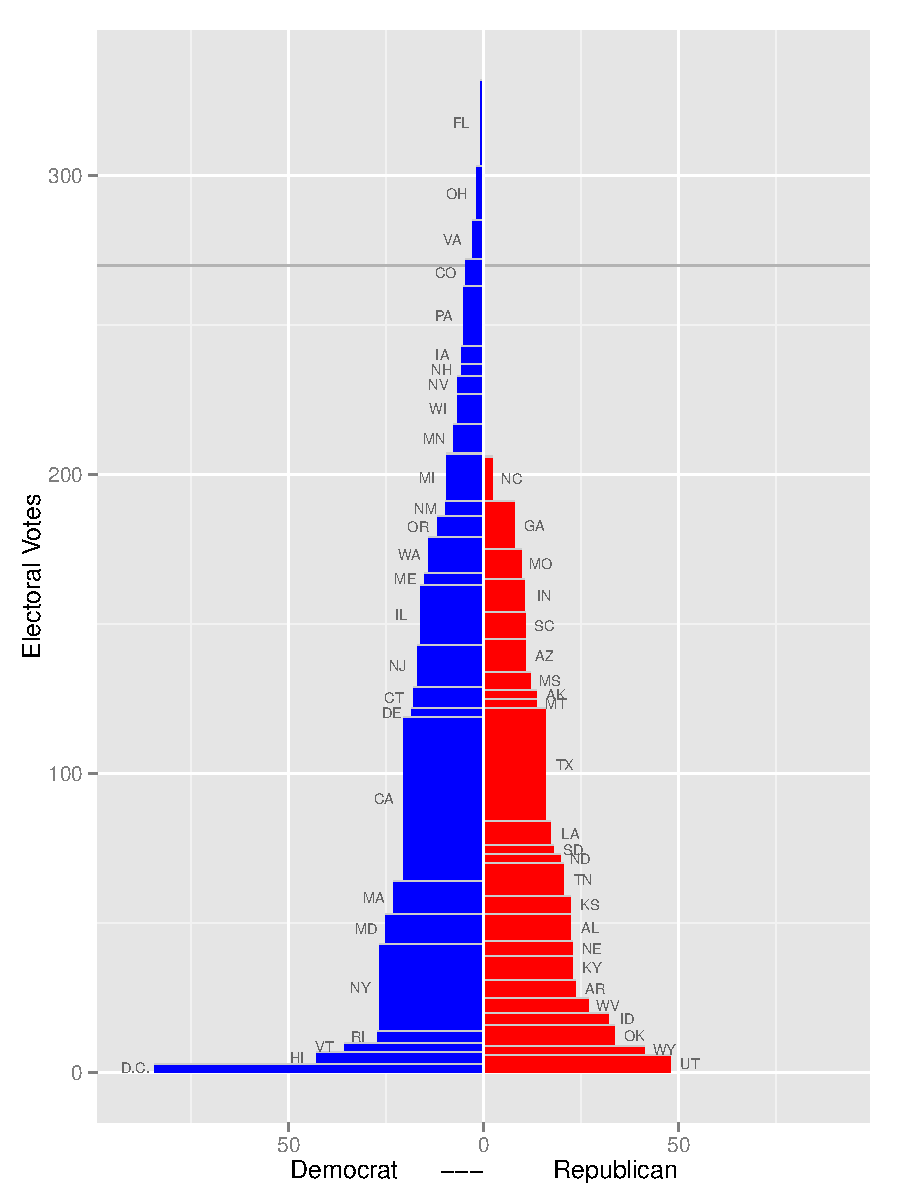
\includegraphics[width=\textwidth]{tower.pdf}
%    \end{minipage}
%     \hfill
%    \begin{minipage}[c]{0.45\textwidth}
%    Poll aggregator 1 \\
%       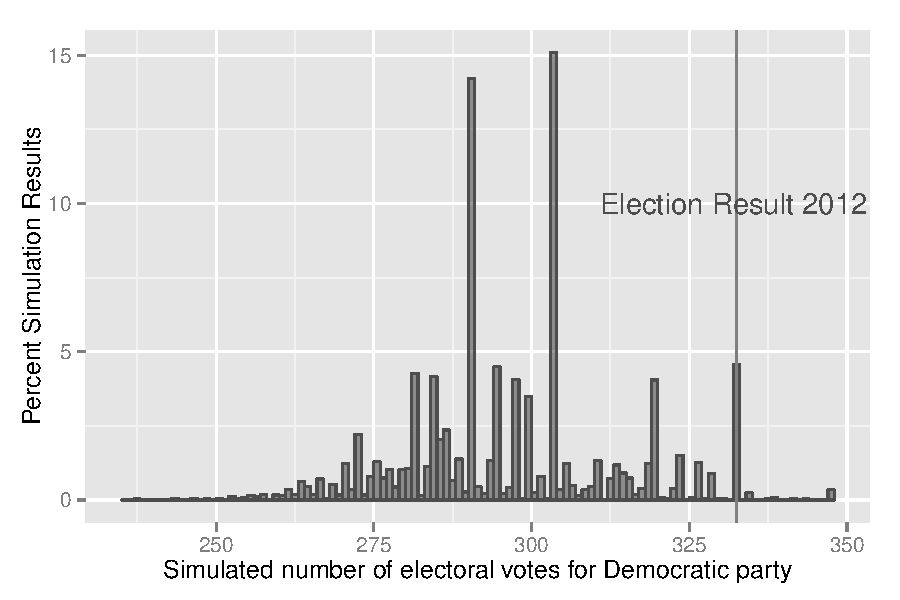
\includegraphics[width=\textwidth]{freedom-sim.pdf} 
%    Poll aggregator 2\\
%       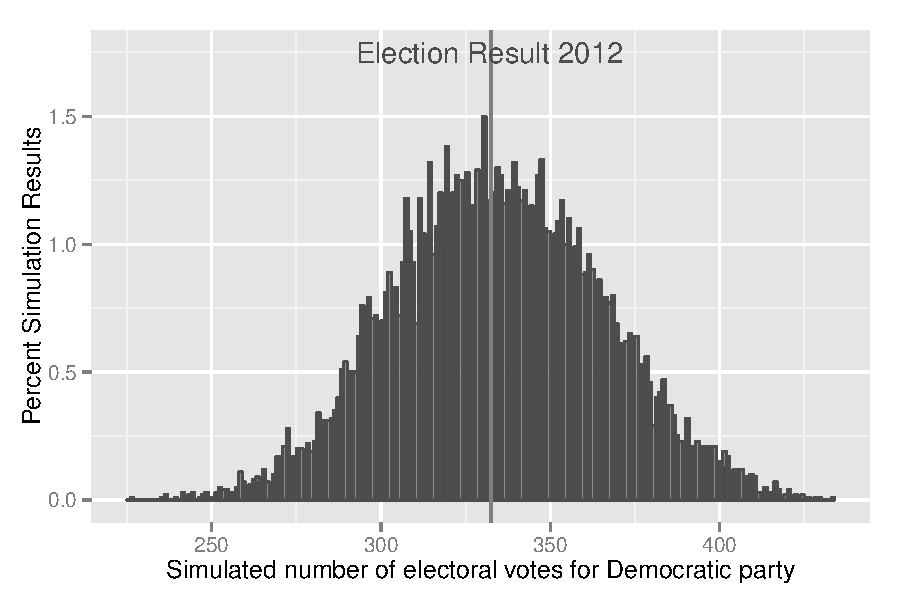
\includegraphics[width=\textwidth]{rcp-sim.pdf} 
%    \end{minipage}
%    \caption{ \label{fig:tower} Electoral building plot of the results of the 2012 U.S. Presidential Election (left). On the right two histograms showing simulated poll results for the Democratic presidential candidate using  polling averages collected from two different sources, Freedom's Lighthouse Averages (top), RealClearPolitics (bottom).  If the polls matched the electoral result the simulated results would be centered at the electoral result. This happens for the RealClearPolitics polls (bottom) but not for Freedom's Lighthouse.  For the latter, only 5.33\% of simulated results were as high as the actual election result, which converts to a $p$-value of 0.0533, indicating an almost statistically significant difference. It hints at the polls from this source under-estimating the vote for Obama. This source was used to generate the null plots in the lineup in Figure~\ref{fig:elect}. The $p$-value from the lineup protocol, was 0.0077, which more strongly concludes that these polls mismatched the actual result.}
%\end{figure}
%The lineup of Figure~\ref{fig:elect}, as well as the other lineups in the manuscript are created using the nullabor package by \citep{nullabor}.

%A lineup can be evaluated by a single person or multiple observers. A distribution similar to the binomial distribution, but adjusted for dependencies introduced by the lineup scenario, is used to calculate the $p$-value based on the number of times observers identify the actual data plot, which provides the information needed to make a decision on rejecting or failing to reject the null hypothesis \citep{vinference}.  To avoid expectation errors \citep{meilgaard}, particularly in emotionally charged areas such as election results, observers should not be aware of the data that constitutes a lineup, and should therefore not have seen the actual data plot before inspecting the lineup. This is the reason that we revealed the context of the election problem only after the interested reader had a chance to evaluate the lineup. 

%When presenting a lineup to an observer the accompanying question should be phrased in as general a manner as possible, effectively asking the observer to pick the plot that is most different, and allowing observers to provide their own reasons for their choice. This ensures all possible deviations from the null hypothesis to be detected. However, if lineup tests are run in head-to-head comparisons with conventional statistical tests, such as the experiments in \cite{majumder:2013} or \cite{tengfei:2013}, these questions have to be phrased much more specifically, in order to avoid  type III errors \citep{mosteller:48} consisting of correctly rejecting the null hypothesis for a wrong reason. In those experiments, the structure in the data is strictly controlled in the simulation process, which allows for specific questions to be asked. 

A lineup can be evaluated by one or more observers, and a distribution similar to the binomial, adjusted for dependencies from the lineup scenario, is used to calculate the $p$-value based on how often the actual data plot is identified \citep{vinference}. To avoid expectation bias \citep{meilgaard}, especially in sensitive areas like election results, observers must not know the data constituting the lineup or have seen the actual data plot beforehand. The context of the election problem was revealed only after lineup evaluation to prevent bias. The accompanying question in a lineup should be broad, asking observers to pick the most distinct plot, allowing detection of any deviations from the null hypothesis. However, in head-to-head tests with conventional methods \citep{majumder:2013, tengfei:2013}, specific questions are needed to avoid type III errors \citep{mosteller:48} consisting of correctly rejecting the null hypothesis for a wrong reason.


%In the election example, observers were asked ``which plot is the most different?''. The type of plot, showing two (modified) stacked bar charts in different colors should suggest to the observer that the interesting feature is the difference between the two heights. Most observers based their decision on this -- besides  `asymmetry' between the towers (a reason suggested by us), most free-form responses for the reason of choice describe a comparison between the red and blue towers. In the responses for this lineup we see something that is very typical of responses in lineups: it is only a few panels from the lineup that observers pick, while most panels do not get picked or get picked only a few times. Out of a total of 72~responses, 23 observers picked panel~\#8, 12 observers picked the (data) panel \#13, 10 observers picked panel~\#4, 6 observers picked panel \#7, and all of the remaining panels were picked at most three times. From the panels picked, we see that the top three choices  are all extreme with respect to heights of blue versus red towers:  both panels \#8 and \#13 show a large difference between the height of the towers, while panel \#4 is the only panel, in which the red tower is higher than the blue one. 

The lineup protocols allows us to calculate all relevant properties that we are familiar with from conventional statistical tests. In particular, the power of a lineup is calculated as the {\it detection rate} at which observers identify the actual data plot. Visual power depends unlike power in conventional tests not only on the strength of the signal, but also on individuals' ability. The ability of individual observers varies, and the effects that might influence this ability are the focus of this paper.


%We have conducted a series of experiments (see Table~\ref{tbl:visual_stat} for an overview) using Amazon's Mechanical Turk~\citep{turk} (MTurk) for a variety to purposes: validating the protocol against existing tests, comparing plot designs, and evaluating structure in data analysis problems. In all of the experiments we collected demographic details, such as gender, age bracket, and educational background.  Mining this data will provide a basis for evaluating the effects of different covariates on an individual's ability to evaluate lineups. The design of some of the experiments allow a further investigation into aspects beyond participants' demographics: experiments~5, 6 and 7 can be used to investigate short term learning trends, while experiment~9 allows insight on whether the  positioning of the  data plot in the lineup has an effect on detection rate. 

We conducted several experiments (see Table~\ref{tbl:visual_stat}) using Amazon's Mechanical Turk~\citep{turk} (MTurk) for validating the lineup protocol, comparing plot designs, and evaluating data analysis structures. Demographic data such as gender, age, and educational background were collected to assess the influence of these covariates on lineup evaluations. Additionally, experiments investigated short-term learning trends as well as explored the effect of data plot positioning on detection rates.
 
%Section~\ref{sec:factor_performance} discusses human factors that we expect to be influential on the performance of the observer. Section~\ref{sec:exp_design} describes the methods used to assess the effects, and Section~\ref{sec:result_socio} summarizes the results of what we have learned about human factors affecting lineup evaluation.


Section~\ref{sec:factor_performance} discusses expected human factors influencing observer performance and Section~\ref{sec:result_socio} presents findings on factors affecting lineup evaluations. The methods used to assess the effects are oulined in Appendix~\ref{sec:exp_design}. 



% ===================================================================================
\section{Factors Potentially Affecting Visual Inference} \label{sec:factor_performance} 
%------------------------------------------------------------------------------------

Visual statistical inference relies not only on the strength of the signal in the data, but also on how this information is presented in the plot, on the lineup design and on the abilities of human observers. It is important to understand how these factors might affect results.  Here, we provide a brief discussion %This section provides a brief description 
of the factors that are expected to have some impact on the performance of visual statistical inference.  


\begin{itemize} \itemsep 0in \parsep-10pt %\parskip0pt 
 
%\item{\bf Choice of Visual Test Statistic:}  
%Data can be plotted in a variety of ways and we can enhance plots by axes, legends or representations of models. The choice of plot primarily should be appropriate for the problem being investigated, as the data plot is the visual test statistic. 
%When for example studying the association between two quantitative variables a scatterplot is usually considered best practice. Enhancements, such as a line overlaying a scatterplot to represent a fitted model, might be appropriate for studying models for the data.  Some choices of visual test statistics provide better results than others when studying the same problem \citep{heike:2012}, because some plot types make it easier for certain structures to be seen. 

%Table~\ref{tbl:visual_stat} shows the large variety of visual test statistics used in the Turk studies completed so far. These experiments were conducted to examine many different visual tasks. Side-by-side boxplots were used in experiment~1 to study the importance of a categorical variable in a regression model. For both experiments~2 and~3, a scatterplot is the visual test statistic, but a regression line fitted through the points is overlaid for experiment~2. The experiments studied slightly different problems, for which the difference in plot type was important. Experiment~4 compared polar coordinates to euclidean coordinates on the reading of structure in a barchart.  Experiment~5 examined the style of plot for a bivariate data problem, by comparing results when using a scatterplot, side-by-side dot plots, overlaid densities or side-by-side boxplots. Experiment~6 studied the difference between variations of boxplots. Experiment~7 studied the effects of high dimension low sample size on the separation of groups in low-dimensional projections. The sine illusion, where people read the strength of differences between curves as different when there is a strong sinusoidal structure, is examined in experiment~8. Experiment~9 was conducted to test if there was any structure in an RNA-seq data set measured on soybeans, and used interaction plots classically constructed to examine interaction effects in $2\times 2$ factorial designs. Experiment~10 used different sorts of residual plots for hierarchical linear models as the visual test statistics. 

%In experiments~4,~5 and~6, different visual test statistics were used on the same data, providing the ability to examine the effect of these choices, the use of lineup tests for comparisons and  examples are discussed in \citet{heike:2012, qqplots:2015} 


%\item{\bf Signal in the Data:}
%A visual test statistic is chosen for a particular task. If it is well-designed  departures from the null hypothesis will be visible in the plot, especially if the signal is strong. An important factor that helps an observer to identify the actual data plot in a lineup is the strength of the signal in the data. Simulated data was generated for all of the experiments, except exps.~4 and~9, enabling the study of signal strength and actual data plot detection. In experiment~4 we took a different approach by varying the sampling size, which also allowed us to investigate the effect a design had on detection rate while varying signal/noise ratio. Primarily the results were as expected, that as the signal strength increased observers more frequently picked the actual data plot as different from the null plots. 

%\item{\bf Question Design:} A primary purpose of visual inference is to preclude the necessity to pre-specify discoverable features in data that is required by classical statistical inference. Visual inference supports discovery of structure, enabling the unexpected to surprise us.  This is tightly connected to the task that the human observer is asked to perform. For most purposes the observer is asked a very general question, such as to pick the plot that is most different from the others, and explain the reasons why they see it as different. By being general, all possible discoverable structures are included in the significance calculations \citep[see also ][]{buja:2009}.

%In the initial Turk experiments (1,2,3) conducted with simulated data to compare the results from visual inference with those obtained by classical inference, the questions posed to the observers were more targeted. This was important to allow a direct comparison of the results to those from conventional testing. %in order to make a comparison of the results. 
%For latter studies (4, 7, 10), questions posed to the observer were more general. Table~\ref{tbl:visual_stat} lists the questions used for each experiment. 


\item{\bf Demographics:}  During each of the experiments, data on age, gender, education level and geographic location was collected. Each observer self-reported gender, age in roughly five year intervals, education level as high school or less, some college courses, an undergraduate degree, some graduate courses or a graduate degree. The IP address of the computer afforded the geographical location of the subject. The purpose of collecting this information with each experiment is to examine the effect that they have on the results of visual inference -- ideally very little. 

\item{\bf Learning Trend:} One might expect that as an observer evaluates more lineups they  become more skillful in their evaluations. Each participant in  experiments~5, 6 and~7 was asked to evaluate a block of  ten lineups of the same type of data plot. The ten lineups were randomly chosen from the lineups  produced for each study. Before evaluating the first lineup, the observer needs to read instructions and become accustomed to the type of plot used in the lineup. In subsequent lineups  the type of plot is the same. It is possible that the observer becomes more skillful at recognizing the most different plot, either by more often detecting the actual data plot or more quickly reporting their choice. These two ways of measuring learning trend are evaluated on data collected from experiments~5, 6 and~7.


%\item{\bf Location of Actual Data Plot in the Lineup} For all of the lineups used in the experiments a $5\times 4$ grid of 20 panels is used. A random number generator is used to determine the position where the actual data plot is placed in each lineup. Eye tracking experiments \citep{zhao:2012} suggest that some observers traverse lineups in horizontal direction, while others have a vertical up-and-down approach to their search. Almost universally, observers start at the top left of a lineup. This leads to some concern that observers might be able to more easily identify the actual data plot, if it is placed at the top left of a lineup than when it the actual data is placed at the bottom right.

%Ideally, this does not happen. Experiment~9  is designed to allow us to investigate the effects of location on detection. Five different locations in the lineup were used to assess how fast and accurately observers identified the actual data plot.


%\item{\bf Sample of Null Plots:} In classical inference, the test statistic is compared to the full null distribution, to decide if it is extreme or not. In visual inference the actual plot is compared to plots of a finite number of samples from the null distribution. In the lineups used in the Turk experiments, the actual data plot is compared on 19 null plots. These null samples are random draws, and there is a chance that one or more null plots in the lineup may be similar or even more extreme than the actual data plot. The sample of null plots can affect the observer's decision. This is tested with the data from experiment~9, where the experiment was set up with lineups made from different null plots.

%\subsection{Individual Skill or Ability} 
\item{\bf Individual Skill or Ability:} Each person may have different  aptitude for reading statistical plots, and their visual skill sets might be differently developed.  We can examine the effect of individuals' skills and abilities because multiple subjects evaluated the same lineups, which allows us to estimate, if some subjects consistently detect the actual data plot more often than others.  
 %For example, in a controlled experimental study \citet{zhao:2012}  noticed that some people spent a lot of time to decide no matter whether the lineup is difficult or easy while some simply glanced at lineups to make a decision. This influences the response of the observer. Also subject specific variation in the power of visual test is observed in \cite{majumder:2013}. 
\end{itemize}


% 
% % ===================================================================================
% \section{Experimental Methods}\label{sec:exp_design}
% %------------------------------------------------------------------------------------
% 
% Two of the factors, signal in the data and individual abilities, were studied in \cite{majumder:2013}. The choice of visual test statistic was examined in \cite{heike:2012}. In each of these analyses demographic factors were given a cursory glance, to ensure that they did not have large effects on the results. The design of experiments 5, 6 and 7 enables the examination of learning trend, which is studied in this paper. Experiment~9 was a real test case for visual statistical inference, and in order to understand the significance of the structure in the genomic data, multiple lineups were made in which location of the actual data plot, and the sample of nulls, were randomized. This enables the assessment of the effect of these factors on the results. This section describes the experimental methods used to examine the effects of demography, placement of the actual data plot, sample of null plots and the existence of a learning trend. 
% 
% \subsection{Demographic Factors}
% \noindent
% For all  ten experiments shown in Table~\ref{tbl:visual_stat}, the following demographic information was collected from subjects:
% 
% \begin{enumerate} \leftmargin 5cm  \itemsep 0in
% \item {\it Age group}, with categories set to be 18-25, 26-30, 31-35, 36-40, 41-45, 46-50, above 50.
% \item {\it Gender}, male or female.
% \item {\it Education level}, with levels being high school or less, some undergraduate courses, undergraduate degree, some graduate courses, and graduate degree.
% \item {\it Geographical location}, collected from the IP address of the participants' computer, as latitude, longitude, city and country. 
% \end{enumerate}
% 
% 
% Let $Y_{ij}$ denote the response from observer $i$ on a lineup $j$, with $Y_{ij} =1$ if the actual data plot is chosen, otherwise $Y_{ij} =0$. The factors are examined in association with the observer's response using a logistic regression with random effect terms:
% 
% \begin{equation} \label{eqn:demographic_response}
% g( \pi_{ij} )= \mu + \alpha_{k(i)} + \gamma_{l(i)} + \tau_{m(i)}+ \kappa_{s(i)} + \ell_j,  
% \end{equation}
% 
% where $\pi_{ij}=  E(Y_{ij})$ is the probability that  observer $i$ picks the actual data plot from lineup $j$, $\mu$ is an overall population average, $\alpha$, $\gamma$, $\tau$ and  $\kappa$ are the effects of age group $k(i)$, gender $l(i)$, education level $m(i)$ and country name $s(i)$, respectively, for observer $i$. The term $\ell_j$ is a random intercept predicting lineup difficulty level and we assume independence and normality of the errors, i.e.\ $\ell_j \sim N(0, \sigma_\ell^2)$.  $g(.)$ denotes the {\it logit} link function $g(\pi)=\log(\pi) - \log(1-\pi); 0 \le \pi \le 1$.
% 
% 
% Similarly, we model the  time  an observer takes to identify a panel from a lineup. Let $Z_{ij}$ denote the logarithm of time taken for  observer $i$ to evaluate  lineup $j$. Let $\mu_{ij}=  E(Z_{ij})$ be the average of the (log) time taken by  observer $i$ to pick a panel from lineup $j$. We model this in a mixed effects model of the same structure as model~(\ref{eqn:demographic_response}) given as:
% %\hh{
% \begin{equation} \label{eqn:demographic_time}
% Z_{ij} = \mu + \alpha_{k(i)} + \gamma_{l(i)} + \tau_{m(i)}+ \kappa_{s(i)} + \ell_j+ \epsilon_{ij},  
% \end{equation}
% where $\mu$ represents overall average of log time taken by an observer to evaluate a lineup, $\alpha$, $\gamma$, $\tau$ and  $\kappa$ are as described in model~\eqref{eqn:demographic_response}, $\ell_j$ is a lineup-specific random effect for the time needed to evaluate a lineup, with $\ell_j \sim N(0, \sigma_\ell^2)$ and the overall error $\epsilon_{ij} \sim N(0, \sigma^2)$.  
% 
% \subsection{Learning Trend} Learning trend of a subject can be observed in terms of performance over successive responses when multiple lineups are shown for evaluation. Experiments 5, 6 and 7 were used for this. Each subject was shown a total of 10 lineups randomly selected from a pool of lineups. The lineups are not necessarily of the same difficulty level, but the order of lineups was randomized. The responses of the lineups were recorded by attempt 1 through 10. Attempt 1 means that the response is for the first lineup the observer evaluates and attempt 10 refers to the response for the 10th lineup. The goal is to estimate whether performance of the observer improves, or changes, from attempt 1 to attempt 10. 
% 
% It should be noted that we are examining the observer's performance, when we model response as detected or not, but this is not the goal of visual inference. Visual inference is constructed to measure the significance of structure discovered in data. It is expected that some observers will be more skilled at reading data plots, and hence, more readily detect the plot that is different. It is also expected that as observers gain experience in evaluating lineups that they become more proficient in reading data plots, particularly if feedback is given on whether the actual data plot was chosen or not. Choosing the actual data plot will be more difficult in some lineups than others, and indeed should happen purely by chance in some lineups. So in this context, detected, or not, is used as a response to examine individual differences. 
% 
% Let $Y_{ijk}$ denote the response from observer $i$ on lineup $j$ at their $k$th evaluation attempt, where $Y_{ijk}=1$ if the observer detected the actual data plot otherwise  $Y_{ijk}=0$. Let $\pi_{ijk}=  E(Y_{ijk})$ be the probability that  observer $i$ picks the actual data plot from lineup $j$ in their $k$th attempt. Learning trend is assessed using a generalized mixed effects model of the form
% \begin{equation} \label{eqn:trend_response}
% g( \pi_{ijk} )= \mu + \alpha_k + u_i +  a_{i} k + \ell_j,  
% \end{equation}
% where $\mu$ is an overall population average, $\alpha_k$ is the effect of the $k$th attempt on the probability, using the first attempt as reference, $\alpha_1 = 0$, and $k = 1, ..., K$, $u_i$ and $a_i$ are observer specific random effects, $i = 1, ..., I$. The term, $u_i$ is a random intercept, describing a basic subject-specific ability, with $u_i \sim N(0, \sigma_u^2)$. 
% The term $a_i$ is a random slope capturing an individual's specific learning effect over the course of $K$ attempts, where $a_i \sim N(0, \sigma_a^2)$. 
% For $\ell_j$ a normal distribution, $N(0, \sigma_\ell^2)$, is assumed, and $\ell_j$ is a random intercept predicting lineup difficulty level. $g(.)$ denotes the {\it logit} link function $g(\pi)=\log(\pi) - \log(1-\pi); 0 \le \pi \le 1$. The inverse link function, $g^{-1}(.)$, from equation~\ref{eqn:trend_response} leads to the estimate of the subject and the lineup specific probability of successful evaluation in the $k$th attempt by a single observer as 
% \begin{equation} \label{eqn:trend_power}
% \hat p_{ijk} =  g^{-1}(\hat{\mu} + \hat{\alpha}_k + \hat{u}_i +  \hat{a}_i k + \hat{\ell}_j).
% \end{equation}
% 
% When time taken to evaluate a lineup is used as the response, let $Z_{ijk}$ denote the logarithm of time taken for an observer $i$ to evaluate a  lineup $j$ in his/her $k$th attempt. Let $\mu_{ijk}=  E(Z_{ijk})$ be the average of the (log) of time taken by  observer $i$ to choosing a  panel from lineup $j$ in his/her $k$th attempt. We evaluate this in a mixed effects model of the form
% 
% \begin{equation} \label{eqn:trend_time}
% Z_{ijk} = \mu + \alpha_1 + \alpha k + u_i +  a_{i} k + \ell_j + \epsilon_{ijk},  
% \end{equation}
% where $\mu$ represents overall average of log time taken by an observer to evaluate a lineup, $\alpha$ is the average change in log time taken for each additional attempt,  $\alpha_1$ is an offset in log time taken for the first attempt. All other effects are random effects: $u_i$ is a subject-specific intercept representing individual speed of an observer with $u_i \sim N(0, \sigma_u^2)$, $a_i$ is a subject-specific slope representing the deviation of the speed-up (or -down) by attempt $k$, with $a_i \sim N(0, \sigma_a^2)$, $\ell_j$ is a lineup-specific random effect for the time needed to evaluate a lineup, $\ell_j \sim N(0, \sigma_\ell^2)$ and the overall error $\epsilon_{ijk} \sim N(0, \sigma^2)$.
% Equation~\ref{eqn:trend_time} leads to the estimate of the subject and the lineup specific time taken for an evaluation in $k$th attempt by a single observer as 
% \begin{equation} \label{eqn:trend_time_est}
% \hat \mu_{ijk} =  \hat{\mu} + \hat{\alpha_1}+ \hat{\alpha}k + \hat{u}_i +  \hat{a}_i k + \hat{\ell}_j.
% \end{equation}
% 
% To fit all these mixed effect models the function {\tt lmer()} is used from R package {\tt lme4} by \cite{lme4:2015, lme4:paper}. We employ a normal approximation to obtain $p$-values corresponding to fixed effect parameters estimates.  
% 
% \subsection{Location Effect} \label{sec:location_design} Experiment~9 studied significant expression in an RNA-seq study, and was designed so that location effect of the actual data plot in a lineup could also be assessed. The data used, documented in \cite{atwood:2013}, measures gene expression of soybean by RNA-seq methods. Two factors were of primary interest a main effect for genotype and an interaction effect between genotype and treatment condition.
% 
% In large studies such as this there is a valid question whether the data exhibits any structure at all, or if the small $p$-values are simply occurring by chance, from the massive multiple testing. This overall significance is studied using visual inference  in \citet{tengfei:2013}. 
% 
% In order to study the effect that  location has on evaluating lineups, we used multiple lineups for each of the data plots. For each data plot, five sets of null plots were generated and the actual plot was randomly placed in one of five different locations in a lineup of size 20. 
% For the genotype effect, the locations were  1, 8, 12, 17, 20 and locations 2, 9, 12, 16, 20 were used for the interaction effect. %Five different sets of null plots were used to produce 5 lineups for each location position, creating 
% Overall this created a total of 25 lineups for studying the genotype effect, and another 25 lineups for studying the interaction effect. Each observer saw three lineups, one for genotype, one for interaction, and one easy lineup that was used to help clean the data. 
% 
% To examine if the difference in detection rate among the locations is statistically significant a one-way multivariate analysis of variance (MANOVA) model is fit to the data.
% Let $\mathbf{Y}=(Y_1,Y_2, ... , Y_p)^\top$ be a vector of random variables with dimension $p = 5$, the total number of null sets, and let $\mathbf{Y}_{ij}$ represent the $j$th vector response for  location $i$ with $i=1,2, ..., I$ for $U=5$. Because the same data plot is shown in each lineup, it is assumed that there could be some association between the responses for each null set, which suggests the MANOVA model rather than a univariate ANOVA.  The MANOVA model 
% \begin{equation}\label{manova}
% \mathbf{Y}_{ij} = \mu_{i} + \epsilon_{ij}
% \end{equation}
% where $\mu_{i}= (\mu_{1i},\mu_{2i}, ..., \mu_{pi})^\top$ is the mean vector for location $i$ and $Var(\epsilon_{ij})=\Sigma$, tests for significant difference between the means. 
% 
% \subsection{Data Collection Methods}  Human subjects were recruited to evaluate the experimental lineups through MTurk \citep{turk}.  It is an online work place where people from around the world can sign up for so-called `HIT's, human intelligence tasks, generally short tasks that are humans are typically better at solving than computers. Usually tasks are very simple and no specialized training is required to do them. Tasks are designed for anyone to do but some tasks may require some skills depending on the recruiters' need. %Each task is usually planned to completed in a short time.  
%  For completing a HIT workers are paid a small amount of money, on the order of minimum wage in the USA. 
% 
% 
% We designed and developed a web application which enables the display of lineups to  observers as per experimental need. The MTurk workers were re-directed to this web application to complete their assigned tasks. Responses were collected, stored automatically into a local database server, along with demographic information, age group, gender and education level. The time taken for each evaluation is computed based on the time the plot was shown and the time the feedback was received. Location of an observer is determined based on the ip address of the observer.
% 

% ===================================================================================
\section{Results}\label{sec:result_socio}
%------------------------------------------------------------------------------------

 \subsection{Overview of the Data} In ten experimental studies, a total of 2,340 participants from 70 countries, primarily the United States and India, provided feedback data on lineups, ensuring a diverse pool of respondents in terms of geography, gender, age, and education. The demographic details, as summarized in Table~\ref{tbl:turker_location}, revealed a high number of female participants across most countries, which was an unexpected but positive outcome. Notably, countries like Canada, Romania, the United Kingdom, and Macedonia also had notable participant representation.

The majority of participants were aged 18 to 35, with the United States showing a more balanced age distribution compared to India, where younger individuals were more prevalent. Educational backgrounds were diverse, with 38.42\% of participants reporting a graduate degree. However, there was a cultural misunderstanding as Indian participants classified any university degree as a graduate degree, while the North American definition refers to a Master’s degree or higher. Compared to the 2010 US Census \cite{census}, the participants skewed younger and more highly educated.

In total, 1,912 lineups were evaluated across the studies, with each participant reviewing at least 10 lineups, except for experiment~9, where they reviewed three. To ensure quality, participants were given test plots to evaluate first, and incorrect responses led to their data being excluded from the analysis. Some demographic and geographical data were missing due to participants opting out or issues retrieving IP-based location data.

%A total of 2340 participants provided feedback data on the lineups in ten different experimental studies. Figure~\ref{fig:turker_location} displays the locations of participants around the world.  Most of the participants were from the United States and India. There were 70 other different countries represented. This provides a diverse pool of participants. The diversity in not only  geographic but also in gender, age group and education level as can be seen in Table~\ref{tbl:demographics}. The large number of female participants from all countries was a pleasant surprise to us.
% 
% 
% Besides the United States and India, countries such as Canada, Romania, the United Kingdom and Macedonia have more than 10 participants each. The remaining 64 countries have fewer than 10 participants each. The distribution of participants is similar in all ten experiments. 
% 
% 
% 
% The largest number of participants falls within the age group of 18 to 25, with the majority being between 18 to 35. Many older participants also took part in the experiments. 
% The United States shows a more uniform participation beyond age 30,  participants from India are primarily younger. 
% 
% In terms of academic background, the majority of participants had a graduate degree (a total of 899 participants, about 38.42\%). Examining the participants' location in conjunction with the academic background reveals that there is an above average  number of participants from India reporting to have a graduate degree. In retrospect this turned out to be a culturally based misunderstanding, as any university degree in India is considered to be a graduate degree, while the North American definition of a graduate degree refers to a Masters level education or above. Most of the  participants from the U.S. report to have an undergraduate degree or at least have some undergraduate courses. 
% 
% Compared to data from the 2010 US Census \cite{census}, participants were both relatively younger, and more highly educated than the general US population. 
% Being turkers implicitly assures that the participants in these experiments have a relatively high level of technological fluency. In fact, the demographics of participants align somewhat better with demographics of internet users published by
% \citet{pew}.
% 
% The distribution of male and female participants are similar among all age groups except for age group 18-25 in India where the proportion of female participants is lower. The distribution of education levels also differs slightly across countries for this age group. 
% 
% 
% A total of 1912 lineups were evaluated in the ten experiments. Each person evaluated at least 10 lineups except for experiment~9 where each participant evaluated three lineups.
% As a measure to ensure a high quality in the evaluations,
%  a test plot was shown to each observer, and the performance on this test plot was used for screening purposes. 
% Test plots were chosen in a way that any serious attempt at answering the lineup would result in a correct answer.
% Data from participants who gave the wrong answer on the test plot 
% led to the removal of all of their answers from the analysis. 
% Results from test plots were also not considered in any of the analyses.
%  In some cases  participants chose to not provide their demographic information. Also, for some ip address, the actual geographical locations could not be retrieved. This resulted in some missing geographic information.

\subsection{Demographic Factors} 

To explore the significance of the demographic factors model~\eqref{eqn:demographic_response} is fit to the data, with age, country, education and gender as fixed effects. To estimate the significance of each of the factors, reduced models are fit with that factor removed from the model. Table~\ref{tbl:anova_factor} summarizes the results. Except for gender, all of the demographic factors show significant differences in  detection rates.  With respect to time taken, all of the demographic factors are significant. 


% latex table generated in R 3.4.1 by xtable 1.8-2 package
% Wed Oct 18 17:22:24 2017
\begin{table}[hbtp]
\caption{\label{tbl:model_result_demographics}Parameter estimates of models~\eqref{eqn:demographic_time} and~\eqref{eqn:demographic_response} fitted for average log time taken and detection rate, respectively. For time taken all the demographic factors are significant. For detection rate, age group 36-40, rest of the world and graduate degree are significantly different. For gender no difference in performance is observed. Lineup variability is estimated to be very large for model~\eqref{eqn:demographic_response}.}
\centering
\scalebox{.9}{
\begin{tabular}{rrr>{(}r<{,}>{\hspace{-.1in}}l<{)}>{\hspace{-.15in}}l<{}cr>{(}r<{,}>{\hspace{-.1in}}l<{)}>{\hspace{-.15in}}l<{}}
 && \multicolumn{4}{c} {Log Time (model~\ref{eqn:demographic_time})} & &\multicolumn{4}{c} {Detection rate (model~\ref{eqn:demographic_response})}  \\

\cline{3-6} \cline{8-11} 
\multicolumn{2}{c}{{Demographic Factor} \hfill Level} & Est & 2.5\% & 97.5\% &   && Est & 2.5\% & 97.5\% &   \\ 
\cline{3-6} \cline{8-11}
\bf Fixed Effects & Average $\mu$ & 3.16 & 3.12 & 3.20 & *** &   & -0.63 & -0.81 & -0.45 & *** \\ [3pt]
\bf Age Category $(\alpha)$ & 18-25 & \multicolumn{5}{l}{0.00} & \multicolumn{4}{l}{\phantom{-}0.00} \\
&  26-30 & 0.05 & 0.03 & 0.07 & *** &   & 0.03 & -0.06 & 0.13 &  \\ 
&  31-35 & 0.06 & 0.03 & 0.09 & *** &   & 0.12 & 0.02 & 0.23 & * \\ 
&  36-40 & 0.22 & 0.19 & 0.25 & *** &   & 0.29 & 0.17 & 0.41 & *** \\ 
&  41-45 & 0.17 & 0.13 & 0.21 & *** &   & 0.19 & 0.03 & 0.34 & * \\ 
&  46-50 & 0.28 & 0.23 & 0.32 & *** &   & 0.20 & 0.01 & 0.39 & * \\ 
&  above 50 & 0.34 & 0.31 & 0.38 & *** &   & 0.16 & 0.02 & 0.29 & * \\ [3pt]
\bf Country $(\kappa)$& U.S. & \multicolumn{5}{l}{0.00} & \multicolumn{4}{l}{\phantom{-}0.00} \\
&  India & 0.23 & 0.20 & 0.25 & *** &   & -0.19 & -0.28 & -0.10 & *** \\ 
&  Rest of the world & 0.14 & 0.11 & 0.17 & *** &   & 0.06 & -0.05 & 0.18 &  \\ [3pt]
\bf Education $(\tau)$& High School & \multicolumn{5}{l}{0.00} & \multicolumn{4}{l}{\phantom{-}0.00} \\
&  Under grad courses & 0.13 & 0.09 & 0.16 & *** &   & 0.00 & -0.14 & 0.14 &  \\ 
&  Under grad degree & 0.14 & 0.10 & 0.17 & *** &   & 0.16 & 0.03 & 0.29 & * \\ 
&  Graduate courses & 0.02 & -0.02 & 0.06 &  &   & -0.13 & -0.29 & 0.03 &  \\ 
&  Graduate degree & 0.13 & 0.10 & 0.16 & *** &   & -0.04 & -0.17 & 0.09 &  \\ [3pt]
\bf Gender $(\gamma)$& Female & \multicolumn{5}{l}{0.00} & \multicolumn{4}{l}{\phantom{-}0.00} \\
&  Male & 0.08 & 0.06 & 0.10 & *** &   & 0.05 & -0.02 & 0.12 &  \\
\cline{3-6} \cline{8-11}
\bf Random Effects &  lineup $(\sigma_\ell)$& \multicolumn{5}{l}{0.29} & \multicolumn{4}{l}{\phantom{-}2.27} \\ 
                   &  Error $(\sigma)$& \multicolumn{5}{l}{0.69} & \multicolumn{4}{l}{\phantom{-}0.89}  \\ 
\cline{3-6} \cline{8-11}\\
\hline
\multicolumn{10}{l}{Signif. codes:  *** $<$ 0.001 $\le$ ** $<$ 0.01 $\le$ * $<$ 0.05 $\le$ . $<$ 0.1 $\le$ ` ' $<$ 1}
\end{tabular}}
\end{table}



Parameter estimates from the model fits are shown in Table~\ref{tbl:model_result_demographics}. The first level of each factor serves as the baseline for the model. The age group 36-40  has a significantly higher detection rate than the 18-25 age group, and to a lesser extent this is also true for other age groups except for 26-30. Participants from the rest of the world have a similar detection rate to those from the USA, but participants from India show a significantly lower detection rate. Subjects reporting to have  an undergraduate degree had a significantly higher detection rate. For time to respond, all age groups were significantly faster than  18-25 year olds.  Participants from India as well as the rest of the world were faster than US Americans. A higher degree corresponded to longer time, and males were on average faster than females.


\begin{figure}[htbp] 
   \centering
   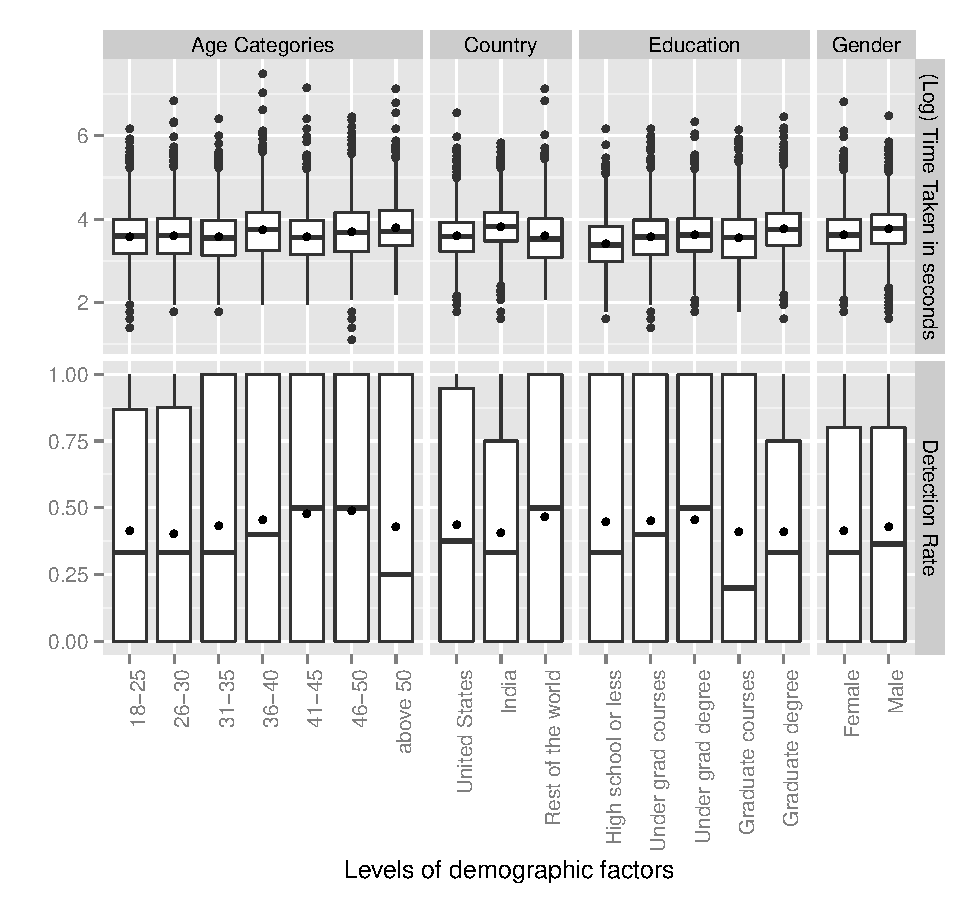
\includegraphics[width=4in]{demographic_effect.pdf} 
   \caption{Boxplots of average log time taken and proportion correct responses (detection rate) of all the lineups plotted for each demographic factor levels. The dots inside the boxes represent means. Some differences in means of various demographic factors are observed. Variability in detection rate indicates large variability in lineup difficulties. }
   \label{fig:demographic_effect}
\end{figure}


Figure~\ref{fig:demographic_effect} supports the model results. The average time taken to respond (natural log) and detection rate are computed by lineup for the different demographic factor levels, and displayed using boxplots. Mean values are shown as dots inside the boxplot, as this statistic rather than the median is used in the models. The means and medians for response time (top row) are essentially equal. There are some differences between the two in the detection rate plots (bottom row). The differences in these values for different factors, that was tested by the models, can be seen in the plots. However, particularly for detection rate, the variation is huge. A large component of the variation is difficulty of the lineup. In some lineups the actual data plot was distinctively different from the null plots, and we would expect that the detection rate would be close to 100\%. In other lineups there was no difference, making it very difficult to evaluate, with low detection rate and longer time to respond. In Table~\ref{tbl:model_result_demographics} notice that lineup specific error is estimated as 2.27 which is much higher than any of the other parameter estimates in the model. This indicates that the major and most important factor affecting the detection rate is  lineup difficulty.  So although the demographic factors emerge from the model to be statistically significant, the practical significance is minimal. We illustrate this with the following example of graduate degree.





While some of the demographic factors are strongly statistically significant, the main source of variation in detection rate is the lineup difficulty. For example, let's examine the effect of an undergraduate degree. To see just how large the effect is, we examine the change in detection rate for a (hypothetical) 18-25 year old female in the United States, with some graduate course work as compared to an undergraduate degree, for an average difficulty lineup (random effect of zero). Plugging in the relevant quantities to the fitted model gives a difference equal to:
$$ \frac {\exp(-0.63-0.13)}{1+\exp(-0.63-0.13)}-  \frac {\exp(-0.63+0.16)}{1+\exp(-0.63+0.16)} = 0.319- 0.385 =-0.066.$$ 
The person with some graduate course work picks the data plot  on average in 31.9\% of lineups of average difficulty, as compared to 38.5\% if they have an undergraduate degree. This difference is reduced to 4\% for a lineup with one standard deviation order of magnitude difference in difficulty. For two standard deviations it further reduces to 0.6\%. Thus, although there is a statistically significant difference in the proportion at which participants identify the  data plot for some demographic factors, these are not  significant in any practical sense.  Figure~\ref{practical_impact_und_und_graduate.pdf} illustrates this example showing fitted models for a US 18-25 female with either a high school education or an undergraduate degree.  Similar calculations show the same negligible impact of age level 36-40 (0.068 at most)  and country India (-0.042 at most) on the probability of a correct response. Thus even though some of the demographic factors are statistically significant, practically, demographics do not substantially influence the results. 

\begin{figure}[htbp] 
   \centering
    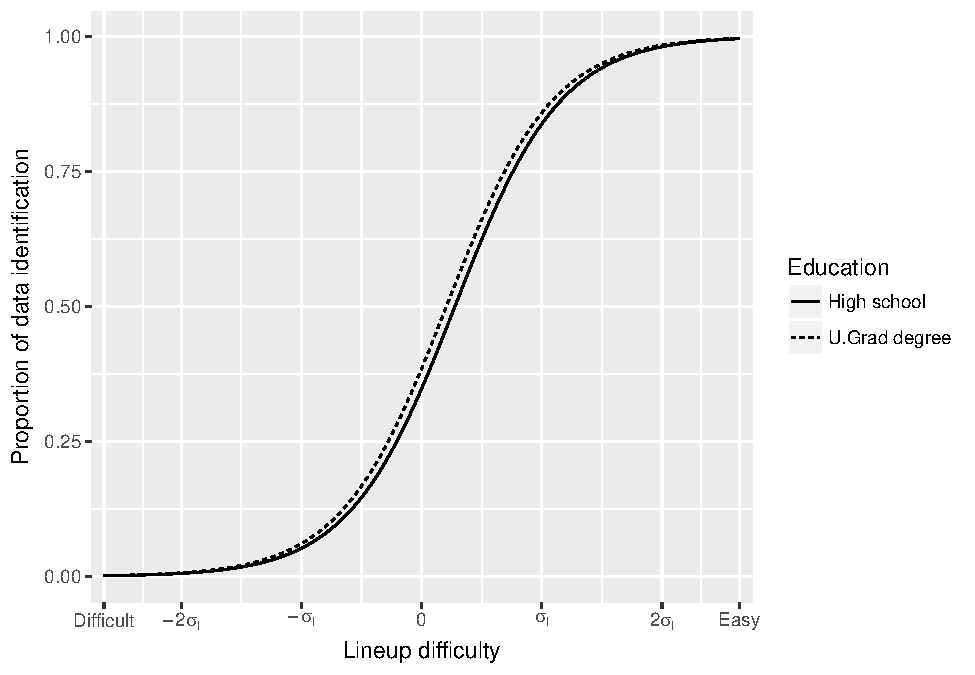
\includegraphics[width=3.2in]{practical_impact_und_graduate.pdf} 
    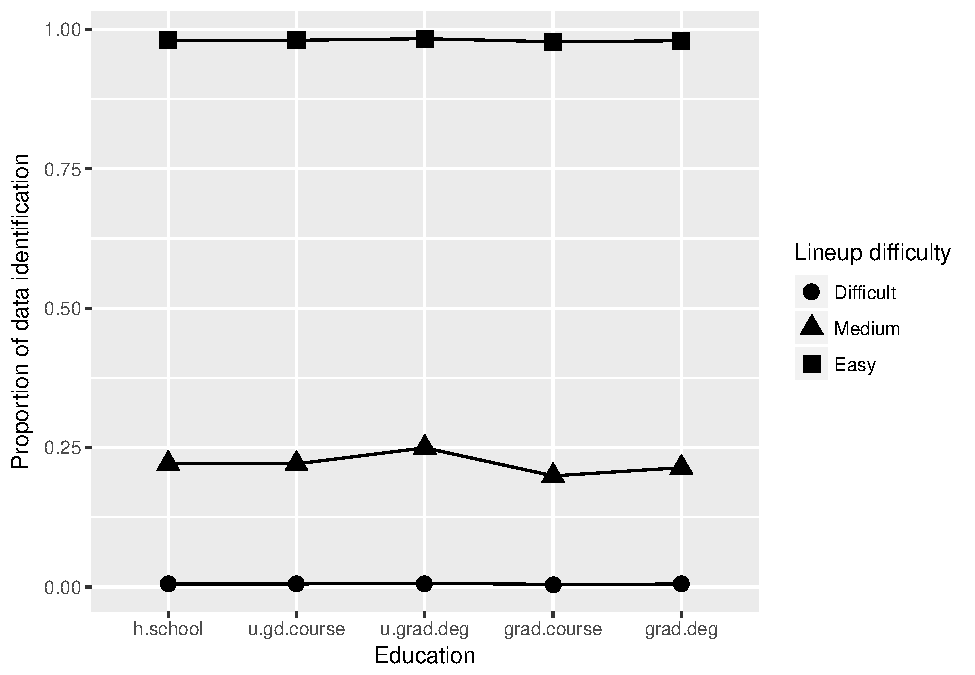
\includegraphics[width=3.2in]{practical_impact_degree.pdf} 
   \caption{Proportion of estimated data identifications by an 18-25 year old female in the United States with an under graduate degree compared to a high school degree. Even though having an under graduate degree leads to  statistically significant increase, the effect size in the dependent variable is  0.04 which is  negligible from a practical point of view. The difference diminishes as we move away one or two standard deviations ($\sigma_{\ell} = 2.27$) 
   of lineup variability.}
   \label{practical_impact_und_und_graduate.pdf}
\end{figure}




\subsection{Learning Trend} Models \eqref{eqn:trend_response} and \eqref{eqn:trend_time} are fitted to the data from experiments~5,~6, and~7 separately. In this model, attempt is fitted as a factor variable to allow for all possible non-linear learning trends.  It should be noted that we also examined an alternative to model~\eqref{eqn:trend_response} where attempt was linearly fitted as a continuous covariate, but this also was not significant.

Table~\ref{tbl:model_result_response} displays the parameter estimates and $p$-values of fixed effect estimates of model~\eqref{eqn:trend_response} examining detection rate. Only for experiment~6 there is some evidence of a learning curve. There are marginally small $p$-values for most of the attempt levels, and positive parameter estimates, suggesting that more attempts increases detection rate. 


% % latex table generated in R 3.4.1 by xtable 1.8-2 package
% % Wed Oct 18 23:54:25 2017
% \begin{table}[hbtp]
% \centering
% \caption{\label{tbl:model_result_response}Parameter estimates of models \eqref{eqn:trend_response} fitted to data from three different experiments using detection rate as the response to assess learning trend. Attempt number is fitted as a factor to enable modeling any sort of non-linear learning trend. Only experiment~6 shows some evidence of a learning trend, with detection rate essentially increasing as attempts increase.}
% \scalebox{.9}{
% \begin{tabular}{rr>{(}r<{,}>{\hspace{-.1in}}l<{)}>{\hspace{-.15in}}l<{}cr>{(}r<{,}>{\hspace{-.1in}}l<{)}>{\hspace{-.15in}}l<{}cr>{(}r<{,}>{\hspace{-.1in}}l<{)}>{\hspace{-.15in}}l<{}}
% \cline{2-5} \cline{7-10} \cline{12-15} 
% & \multicolumn{4}{c} {Experiment~5} & &\multicolumn{4}{c} {Experiment~6} && \multicolumn{4}{c} {Experiment~7}\\
% \cline{2-5} \cline{7-10} \cline{12-15} 
% Effect & Est & 2.5\% & 97.5\% &  & \hspace{1cm} & Est & 2.5\% & 97.5\% &  & \hspace{1cm} & Est & 2.5\% & 97.5\% &  \\ 
% \cline{2-5} \cline{7-10} \cline{12-15} 
% Fixed \\
% $\mu$ & -1.32 & -1.73 & -0.92 & *** &   & -0.16 & -0.46 & 0.13 &  &   & -1.73 & -2.81 & -0.66 & ** \\ [3pt]
%   $\alpha2$ & 0.30 & -0.17 & 0.78 &  &   & 0.26 & -0.07 & 0.58 &  &   & -0.40 & -1.23 & 0.44 &  \\ 
%   $\alpha3$ & -0.20 & -0.68 & 0.29 &  &   & 0.31 & -0.02 & 0.63 & . &   & -0.15 & -0.99 & 0.68 &  \\ 
%   $\alpha4$ & 0.13 & -0.35 & 0.61 &  &   & 0.34 & 0.01 & 0.66 & * &   & -0.41 & -1.24 & 0.42 &  \\ 
%   $\alpha5$ & 0.35 & -0.14 & 0.83 &  &   & 0.34 & 0.02 & 0.67 & * &   & -0.10 & -0.92 & 0.73 &  \\ 
%   $\alpha6$ & 0.10 & -0.40 & 0.60 &  &   & 0.20 & -0.12 & 0.53 &  &   & 0.03 & -0.84 & 0.89 &  \\ 
%   $\alpha7$ & 0.33 & -0.17 & 0.82 &  &   & 0.11 & -0.22 & 0.43 &  &   & -0.00 & -0.84 & 0.84 &  \\ 
%   $\alpha8$ & -0.01 & -0.51 & 0.50 &  &   & 0.31 & -0.01 & 0.64 & . &   & -0.06 & -0.88 & 0.76 &  \\ 
%   $\alpha9$ & -0.20 & -0.70 & 0.30 &  &   & 0.34 & 0.01 & 0.67 & * &   & 0.21 & -0.67 & 1.08 &  \\ 
%   $\alpha10$ & 0.51 & 0.02 & 1.01 & * &   & 0.19 & -0.14 & 0.53 &  &   & -0.20 & -1.07 & 0.67 &  \\ 
%   Random \\
%   $\sigma^2_u$ & \multicolumn{5}{l}{\phantom{-}0.91}  & \multicolumn{5}{l}{\phantom{-}0.89} & 0.82   \\ 
%   $\sigma^2_a$ & \multicolumn{5}{l}{\phantom{-}0.04}  & \multicolumn{5}{l}{\phantom{-}0.04} & 0.05   \\ 
%   $\sigma^2_l$ & \multicolumn{5}{l}{\phantom{-}1.47}  & \multicolumn{5}{l}{\phantom{-}1.43} & 3.38   \\ \cline{2-5} \cline{7-10} \cline{12-15} 
% \\
% \hline
% \multicolumn{10}{l}{Signif. codes:  *** $<$ 0.001 $\le$ ** $<$ 0.01 $\le$ * $<$ 0.05 $\le$ . $<$ 0.1 $\le$ ` ' $<$ 1}
% \end{tabular}}
% \end{table}

% 
% 
% % latex table generated in R 3.4.1 by xtable 1.8-2 package
% % Wed Oct 18 23:54:25 2017
% \begin{table}[ht]
% \centering
% \begin{tabular}{rrrrllrrrllrrrl}
%   \hline
%  & Est & LB & UB & pvalue & g1 & Est.1 & LB.1 & UB.1 & pvalue.1 & g2 & Est.2 & LB.2 & UB.2 & pvalue.2 \\ 
%   \hline
% $\mu$ & -1.32 & -1.73 & -0.92 & *** &   & -0.16 & -0.46 & 0.13 &  &   & -1.73 & -2.81 & -0.66 & ** \\ 
%   $\alpha2$ & 0.30 & -0.17 & 0.78 &  &   & 0.26 & -0.07 & 0.58 &  &   & -0.40 & -1.23 & 0.44 &  \\ 
%   $\alpha3$ & -0.20 & -0.68 & 0.29 &  &   & 0.31 & -0.02 & 0.63 & . &   & -0.15 & -0.99 & 0.68 &  \\ 
%   $\alpha4$ & 0.13 & -0.35 & 0.61 &  &   & 0.34 & 0.01 & 0.66 & * &   & -0.41 & -1.24 & 0.42 &  \\ 
%   $\alpha5$ & 0.35 & -0.14 & 0.83 &  &   & 0.34 & 0.02 & 0.67 & * &   & -0.10 & -0.92 & 0.73 &  \\ 
%   $\alpha6$ & 0.10 & -0.40 & 0.60 &  &   & 0.20 & -0.12 & 0.53 &  &   & 0.03 & -0.84 & 0.89 &  \\ 
%   $\alpha7$ & 0.33 & -0.17 & 0.82 &  &   & 0.11 & -0.22 & 0.43 &  &   & -0.00 & -0.84 & 0.84 &  \\ 
%   $\alpha8$ & -0.01 & -0.51 & 0.50 &  &   & 0.31 & -0.01 & 0.64 & . &   & -0.06 & -0.88 & 0.76 &  \\ 
%   $\alpha9$ & -0.20 & -0.70 & 0.30 &  &   & 0.34 & 0.01 & 0.67 & * &   & 0.21 & -0.67 & 1.08 &  \\ 
%   $\alpha10$ & 0.51 & 0.02 & 1.01 & * &   & 0.19 & -0.14 & 0.53 &  &   & -0.20 & -1.07 & 0.67 &  \\ 
%   $\sigma^2_u$ & 0.91 &  &  &  &   & 0.89 &  &  &  &   & 0.82 &  &  &  \\ 
%   $\sigma^2_a$ & 0.04 &  &  &  &   & 0.04 &  &  &  &   & 0.05 &  &  &  \\ 
%   $\sigma^2_l$ & 1.47 &  &  &  &   & 1.43 &  &  &  &   & 3.38 &  &  &  \\ 
%    \hline
% \end{tabular}
% \end{table}
% 
% 


To visualize how  detection rates change over successive attempts, we fitted model~\eqref{eqn:trend_response} excluding the covariates related to attempt from the model and computed the residuals. Least square regression lines were fitted through the subject specific residuals as shown in Figure~\ref{fig:learning_trend_response}. The averages of these residuals for each of the attempts are shown as dots. Two important features were observed; one is subject specific variability and the other is random slope with attempts which indicates subjects specific learning trend. Some subjects show improvement over time and some show the decrease in performance. Although, the model fit experiment~6 suggested a statistically significant learning curve the plots indicates that it is minimal. 

\begin{figure}[htbp] 
   \centering
    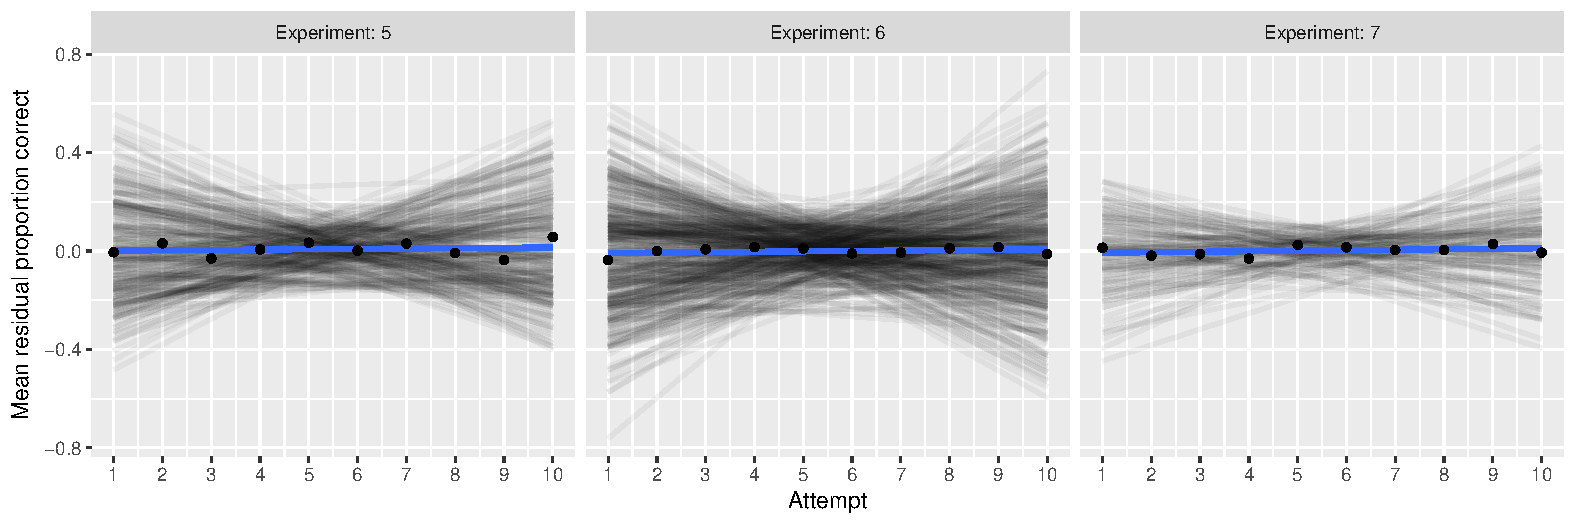
\includegraphics[width=6.3in]{learning_trend_subject.pdf} 
   \caption{ Least square lines fitted through the subject specific residual proportion correct obtained from model~\eqref{eqn:trend_response} fitted without attempt are plotted against attempt. Subject specific positive and negative slopes are observed. Mean residuals are shown as dots and least square regression lines fitted through the points show no overall learning trend in each of the three experiments.}
   \label{fig:learning_trend_response}
\end{figure}


Table~\ref{tbl:model_result_time} presents the results of model~\eqref{eqn:trend_time} where response time is examined with respect to attempt. Attempt is modeled as a linear covariate here, with a shift factor used to adjust for additional time on the first lineup evaluated. Interestingly, time to respond significantly decreases as number of attempts increases, for all three experiments. 
The parameter $\alpha$ for fixed effect covariate attempt is highly significant in all the experiments. The negative estimates suggest that on average later attempts took less time. Even though observers did not improve in their performance in successive attempts, they became more efficient in their response. The parameter $\alpha_1$ for first attempt is also highly significant. The positive estimates of $\alpha_1$ indicates that first attempt made by an observer required much more time than any of the other attempts. One explanation might be that participants take the chance to  carefully read through instructions and familiarize themselves  with the types of plots used in the experiment before evaluating their first lineup, which would inflate the time taken on the first lineup. Each of the experiments asks observers to give a reason for their choice (out of a list of pre-defined answers. For each lineup evaluation, participants are also asked to state how confident in their choice they are (on a scale of 1 to 5).  Later pages of the web site were identical  except for the lineup. 

% % latex table generated in R 3.4.1 by xtable 1.8-2 package
% % Wed Oct 18 23:37:55 2017
% \begin{table}[bhtp]
% \caption{\label{tbl:model_result_time}Parameter estimates of model~\eqref{eqn:trend_time} fitted for log time taken to evaluate a lineup. Both fixed effects parameters of Attempt ($\alpha_1$ and $\alpha$) are highly significant for all three experiments~5,~6 and~7.}
% \centering
% \scalebox{0.9}{
% \begin{tabular}{lr>{(}r<{,}>{\hspace{-.1in}}l<{)}>{\hspace{-.15in}}l<{}cr>{( }r<{,}>{\hspace{-.1in}}l<{)}>{\hspace{-.15in}}l<{}cr>{(}r<{,}>{\hspace{-.1in}}l<{)}>{\hspace{-.15in}}l<{}}
% \cline{2-5} \cline{7-10} \cline{12-15} 
% & \multicolumn{4}{c} {Experiment~5} & &\multicolumn{4}{c} {Experiment~6} && \multicolumn{4}{c} {Experiment~7}\\
% 
% \cline{2-5} \cline{7-10} \cline{12-15} 
% \multicolumn{2}{c}{Effect \hfill Est} & 2.5\% & 97.5\% &  &  & Est & 2.5\% & 97.5\% & &  & Est & 2.5\% & 97.5\% & \\ 
%   \cline{2-5} \cline{7-10} \cline{12-15}
% \multicolumn{2}{l}{Fixed}\\
% $\mu$ & 3.80 & 3.72 & 3.88 & *** &   & 3.89 & 3.83 & 3.96 & *** &   & 3.75 & 3.64 & 3.85 & *** \\ 
%   $\alpha_1$ & 0.32 & 0.25 & 0.39 & *** &   & 0.34 & 0.28 & 0.40 & *** &   & 0.28 & 0.18 & 0.38 & *** \\ 
%   $\alpha$ & -0.04 & -0.05 & -0.03 & *** &   & -0.04 & -0.05 & -0.03 & *** &   & -0.03 & -0.04 & -0.02 & *** \\ 
% \multicolumn{2}{l}{Random}\\
%   $\sigma^2_u$ & \multicolumn{5}{l}{\phantom{-}0.52}   & \multicolumn{5}{l}{\phantom{-}0.49}  & 0.37   \\ 
%   $\sigma^2_a$ & \multicolumn{5}{l}{\phantom{-}0.03}  & \multicolumn{5}{l}{\phantom{-}0.05}   & 0.05   \\ 
%   $\sigma^2_l$ & \multicolumn{5}{l}{\phantom{-}0.09}   & \multicolumn{5}{l}{\phantom{-}0.20}   & 0.24   \\
%   $\sigma^2$ & \multicolumn{5}{l}{\phantom{-}0.46}   & \multicolumn{5}{l}{\phantom{-}0.50}  & 0.45  \\ 
%    \cline{2-5} \cline{7-10} \cline{12-15}
% \end{tabular}}
% \end{table}
% 


% 
% % latex table generated in R 3.4.1 by xtable 1.8-2 package
% % Wed Oct 18 23:37:55 2017
% \begin{table}[ht]
% \centering
% \begin{tabular}{rrrrllrrrllrrrl}
%   \hline
%  & Est & LB & UB & pvalue & g1 & Est.1 & LB.1 & UB.1 & pvalue.1 & g2 & Est.2 & LB.2 & UB.2 & pvalue.2 \\ 
%   \hline
% $\mu$ & 3.80 & 3.72 & 3.88 & *** &   & 3.89 & 3.83 & 3.96 & *** &   & 3.75 & 3.64 & 3.85 & *** \\ 
%   $\alpha_1$ & 0.32 & 0.25 & 0.39 & *** &   & 0.34 & 0.28 & 0.40 & *** &   & 0.28 & 0.18 & 0.38 & *** \\ 
%   $\alpha$ & -0.04 & -0.05 & -0.03 & *** &   & -0.04 & -0.05 & -0.03 & *** &   & -0.03 & -0.04 & -0.02 & *** \\ 
%   $\sigma^2_u$ & 0.52 &  &  &  &   & 0.49 &  &  &  &   & 0.37 &  &  &  \\ 
%   $\sigma^2_a$ & 0.03 &  &  &  &   & 0.05 &  &  &  &   & 0.05 &  &  &  \\ 
%   $\sigma^2_l$ & 0.09 &  &  &  &   & 0.20 &  &  &  &   & 0.24 &  &  &  \\ 
%   $\sigma^2$ & 0.46 &  &  &  &   & 0.50 &  &  &  &   & 0.45 &  &  &  \\ 
%    \hline
% \end{tabular}
% \end{table}


To visualize how the time taken reduces over the successive attempts, we fitted model~\eqref{eqn:trend_time} excluding the covariate attempt from the model and computed the residuals. Least square regression lines are fitted through the subject specific residuals. Subject specific slopes are much different in each of the three experiments as we see in Figure~\ref{fig:learning_trend_time}. Some subjects improved over attempts by taking less time in the later attempts while others got worse. The averages of these residuals for each attempt are plotted as dots. Least square regression lines are fitted to these points excluding the first attempt since for first attempt we fitted an indicator covariate. The downward trends are evident in the plots. All the slopes are highly significant. As expected we observed large positive residuals for each of the experiments for first attempt. 


\begin{figure}[htbp] 
   \centering
%   
\includegraphics[width=6.5in]{learning_trend_time.pdf}    
 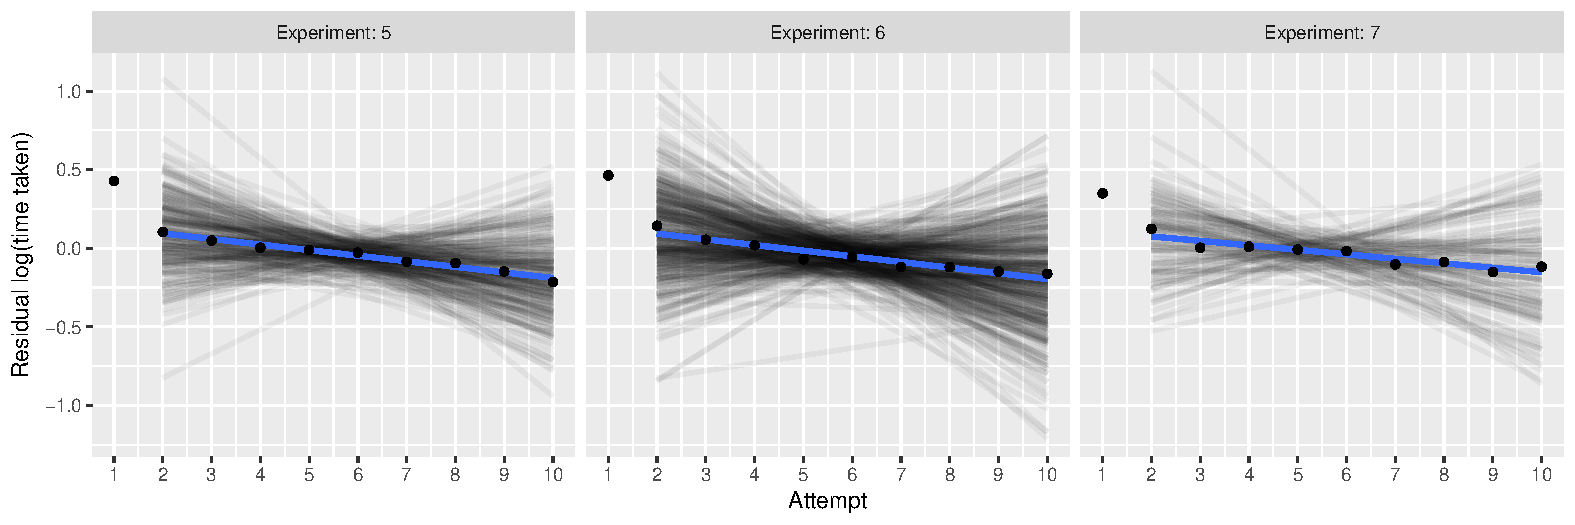
\includegraphics[width=6.3in]{learning_trend_time_subject.pdf}    
   \caption{Least square regression lines fitted through the subject specific residuals obtained by  fitting model~\eqref{eqn:trend_time} without covariate attempt. Differences in subject specific slopes are observed. Some of the subjects did worse over successive attempts while others did better. Averages of these residuals are plotted as dots and least square regression lines are fitted to obtain overall trends. For all the three experiments the overall downward slopes are statistically significant which indicates that MTurk workers become more efficient as they progress through their attempts.}
   \label{fig:learning_trend_time}
\end{figure}

% \subsection{Location Effect}
% 
% A total of 111 subjects was recruited to evaluate lineups designed to investigate the location effect of the actual data plot in the lineup as described in Section~\ref{sec:location_design}. Each subject evaluated two lineups;  one for Interaction effect and the other for Genotype.  In total there were 222 responses for 50 lineups. The data on the test lineup were excluded from the analysis.
% 
% We are investigating location effect in two ways: (1) location effect of each individual plot location, and (2) location effect of inside/outside panel positions.
% 
% Figure~\ref{fig:location_effect} shows an overview of detection rates for both of the effects studied in experiment~9. Each dot corresponds to one lineup. The size of each dot gives the number of evaluations. Lineups with  the same set of null plots are connected by lines.  
% %The detection rate for each data plot location is shown in colored by null sets. 
% The overall average detection rate for each location is shown using dashed lines. Size of the points represent the number of responses. For some locations we have as many as 10 responses. For location 1, we did not have any responses for null set 1 in one of the interaction lineups.
% 
% We observe some variability in the performance due to different null sets even though the same actual data plot was used for all of  these null sets. The lineup protocol is using a finite, small sample (19 in these experiments) of all possible null sets, so it is possible to see some variability in performance depending on the null set. If null sets come from the ``extremes'' of the sampling distribution they may have structure that is more extreme than the actual data plot, making the lineup more difficult to evaluate. From the plot we can see that null set 3 appeared to be more difficult in the Interaction lineup, because the detection rate was lower regardless of the position of the actual data plot. This null set effect was tested, and a significant difference was found for null set 3 of the interaction lineup. The rest of the null sets do not show any differences at  a 1\% significance level. 
% 
% 
% \begin{figure}[htbp] 
%    \centering
%     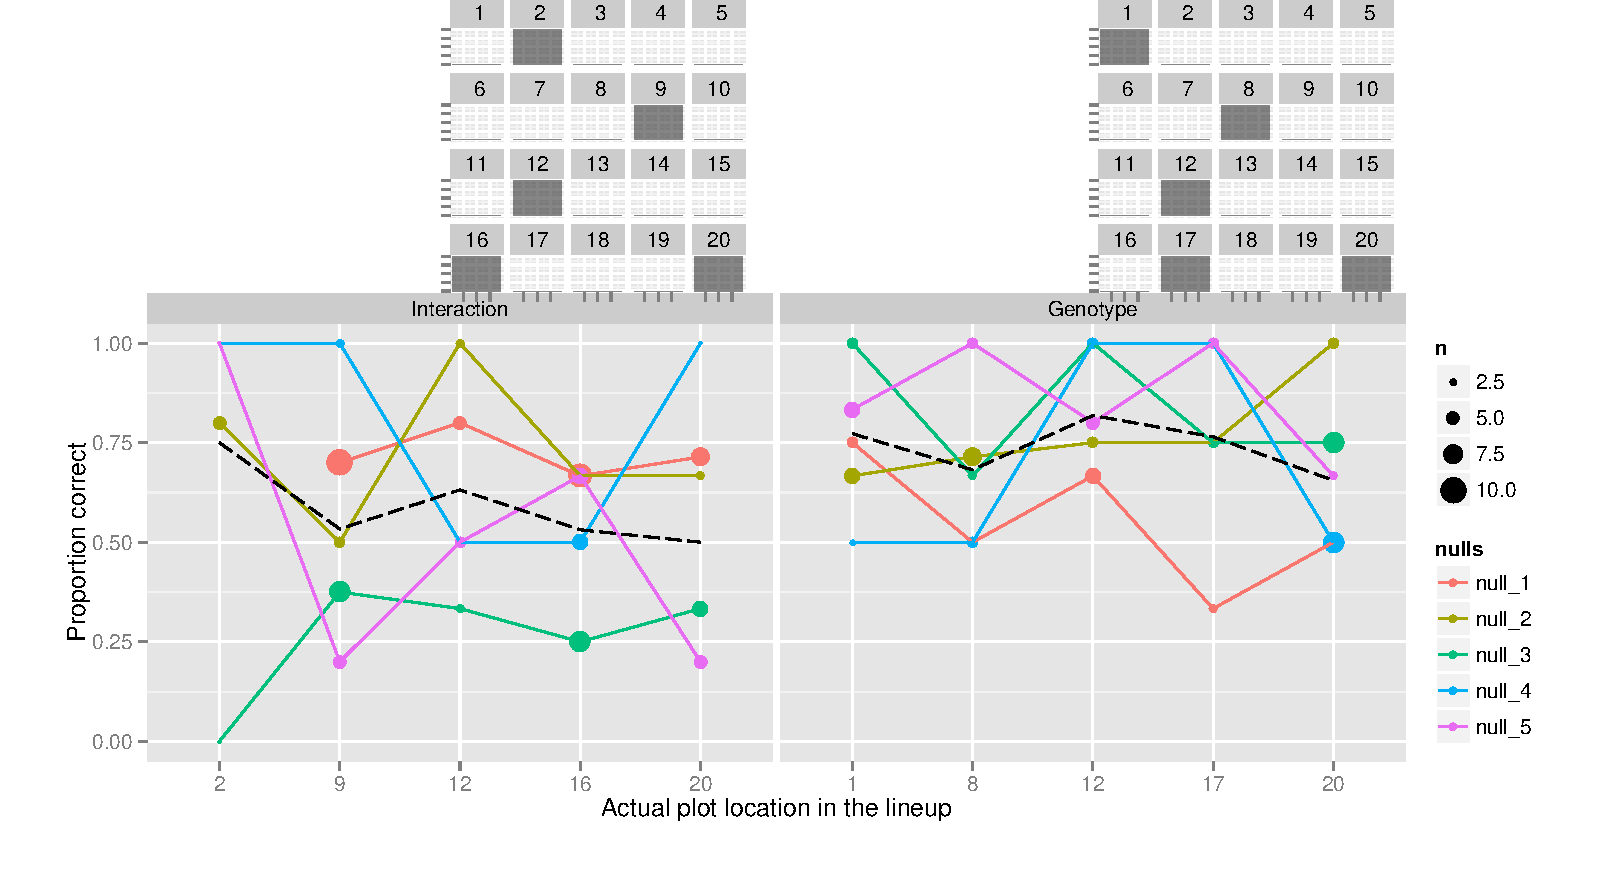
\includegraphics[width=6.5in]{proportion_nulls_guide.pdf} 
%    \caption{Location of data plot in the lineup and proportion correct (detection rate) for both Interaction and Genotype effect. Each colored line represents a null set and the size of the dots represents number of responses. The overall average proportions are shown by dashed lines. The actual data plot locations are shaded grey on the top panels to demonstrate their relative positions on a lineup.}
%    \label{fig:location_effect}
% \end{figure}
% 
% 
% Model~\eqref{manova} was fit to the data to test, if  detection rates were significantly different for the different locations. For this we use the {\it manova()} function provided in the {\it stats} package of the software R \citep{R}. The results are shown in Table~\ref{tbl:manova}. The $p$-values for both the Interaction and the Genotype effect are much bigger than the conventional threshold of 0.05 suggesting that location of the actual data plot in the lineup does not significantly affect performance. 
% 
% \begin{table}[hbtp]
% \caption{The summary of the results obtained by fitting MANOVA model~\eqref{manova} using Wilks test.}
% \begin{center}
% \begin{tabular}{ccccccccc}
%   \hline \hline
%  Location & && & \multicolumn{3}{c} {Degrees of Freedom}  & F test \\
%  \cline{5-7}
%  Effect & DF & Wilks & Approx. F & Numerator& Denominator &Residual & $p$-value\\
%   \hline
%   Interaction& 3&0.07986 & 0.592 &15& \phantom{0}5.92 & 6 & 0.8082 \\ 
%   Genotype & 4&0.01689 & 1.722 & 20&14.22 & 8 & 0.1488 \\ 
%    \hline
% \end{tabular}
% \end{center}
% \label{tbl:manova}
% \end{table}
% 
% For the second approach in investigating the location effect, we distinguish between inner panels 7, 8, 9, 12, 13, 14 and outer panels (any panel with an outside edge). From Figure~\ref{fig:location_effect} we see that location 9, 12 are inner panels for Interaction effect and locations 8, 12 are inner panels for Genotype. Model~\eqref{manova} fitted with two locations effects, inner and outer, did not result in any significant differences.  
 

% ===================================================================================
\section{Conclusion}
%------------------------------------------------------------------------------------

Human demographics have the potential to influence performance when the lineup protocol is used for statistical inference. In our study of the demographic effects on performance across a set of different experiments we found some statistically significant effects. Age group 36-40, people who have a graduate degree have a significantly higher detection rate. India shows significantly lower detection rate compared to United States. Gender does not have any significant effect. However, the effects are minimal, on the order of a few percentage points different from the average. These results are very important for the power of visual tests as they demonstrate the robustness of the test against different human factors.

Individual learning trend is observed in time taken but not so much in observer performance. Some individuals improved on their performances while others showed a decrease on successive attempts. This could be interpreted as good, in the sense that it means that observers could realistically be recruited from sources like MTurk, and that substantial training is not necessary in order to obtain useful evaluations of lineups in practice. However, we had hoped that lineups may be a useful teaching tool, to improve students ability to read data plots, and the lack of a learning trend diminishes this idea, at least for short term learning. 

The simulation experiment reveals that there is no significant effect of location on the actual data plot in the lineup. This is important as the visual statistical inference procedure prescribes that the data plot be placed at random in the lineup. This paper suggests that any random place in a lineup is as good as other places in the lineup. Even though there are variations on the performance depending on different null sets, their impact on probability to correctly evaluate a lineup is very negligible. 

There are many more ways that the lineup protocol might be tested to learn what we might expect about its performance for tackling real data mining problems. Possible changes in the lineup protocol in the pipeline are allowing observers to select more than one plot, and to vary the size of the lineup from 20 to a smaller number, and have observers all see different lineups with different null sets.  This paper assessed the effect of human factors on the experiments conducted to date. As changes to the lineup protocol are suggested by other experiments the human factor effects may need to be examined again.


\if1\blindDoc
{
%------------------------------------------------------------------------------------
\paragraph{Acknowledgments}
%------------------------------------------------------------------------------------
This work was funded in part by National Science Foundation grant DMS 1007697. All studies were conducted with approval from the Institutional Review Board IRB 10-347.
} \fi


\bibliographystyle{asa}
\bibliography{references}



% ---------------------------------------- Appendix ----------------------------------

\appendix


% ===================================================================================
\section{Experimental Methods}\label{sec:exp_design}
%------------------------------------------------------------------------------------

Two of the factors, signal in the data and individual abilities, were studied in \cite{majumder:2013}. The choice of visual test statistic was examined in \cite{heike:2012}. In each of these analyses demographic factors were given a cursory glance, to ensure that they did not have large effects on the results. The design of experiments 5, 6 and 7 enables the examination of learning trend, which is studied in this paper. Experiment~9 was a real test case for visual statistical inference, and in order to understand the significance of the structure in the genomic data, multiple lineups were made in which location of the actual data plot, and the sample of nulls, were randomized. This enables the assessment of the effect of these factors on the results. This section describes the experimental methods used to examine the effects of demography, placement of the actual data plot, sample of null plots and the existence of a learning trend. 

\subsection{Demographic Factors}
\noindent
For all  ten experiments shown in Table~\ref{tbl:visual_stat}, the following demographic information was collected from subjects:

\begin{enumerate} \leftmargin 5cm  \itemsep 0in
\item {\it Age group}, with categories set to be 18-25, 26-30, 31-35, 36-40, 41-45, 46-50, above 50.
\item {\it Gender}, male or female.
\item {\it Education level}, with levels being high school or less, some undergraduate courses, undergraduate degree, some graduate courses, and graduate degree.
\item {\it Geographical location}, collected from the IP address of the participants' computer, as latitude, longitude, city and country. 
\end{enumerate}


Let $Y_{ij}$ denote the response from observer $i$ on a lineup $j$, with $Y_{ij} =1$ if the actual data plot is chosen, otherwise $Y_{ij} =0$. The factors are examined in association with the observer's response using a logistic regression with random effect terms:

\begin{equation} \label{eqn:demographic_response}
g( \pi_{ij} )= \mu + \alpha_{k(i)} + \gamma_{l(i)} + \tau_{m(i)}+ \kappa_{s(i)} + \ell_j,  
\end{equation}

where $\pi_{ij}=  E(Y_{ij})$ is the probability that  observer $i$ picks the actual data plot from lineup $j$, $\mu$ is an overall population average, $\alpha$, $\gamma$, $\tau$ and  $\kappa$ are the effects of age group $k(i)$, gender $l(i)$, education level $m(i)$ and country name $s(i)$, respectively, for observer $i$. The term $\ell_j$ is a random intercept predicting lineup difficulty level and we assume independence and normality of the errors, i.e.\ $\ell_j \sim N(0, \sigma_\ell^2)$.  $g(.)$ denotes the {\it logit} link function $g(\pi)=\log(\pi) - \log(1-\pi); 0 \le \pi \le 1$.


Similarly, we model the  time  an observer takes to identify a panel from a lineup. Let $Z_{ij}$ denote the logarithm of time taken for  observer $i$ to evaluate  lineup $j$. Let $\mu_{ij}=  E(Z_{ij})$ be the average of the (log) time taken by  observer $i$ to pick a panel from lineup $j$. We model this in a mixed effects model of the same structure as model~(\ref{eqn:demographic_response}) given as:
%\hh{
\begin{equation} \label{eqn:demographic_time}
Z_{ij} = \mu + \alpha_{k(i)} + \gamma_{l(i)} + \tau_{m(i)}+ \kappa_{s(i)} + \ell_j+ \epsilon_{ij},  
\end{equation}
where $\mu$ represents overall average of log time taken by an observer to evaluate a lineup, $\alpha$, $\gamma$, $\tau$ and  $\kappa$ are as described in model~\eqref{eqn:demographic_response}, $\ell_j$ is a lineup-specific random effect for the time needed to evaluate a lineup, with $\ell_j \sim N(0, \sigma_\ell^2)$ and the overall error $\epsilon_{ij} \sim N(0, \sigma^2)$.  

\subsection{Learning Trend} Learning trend of a subject can be observed in terms of performance over successive responses when multiple lineups are shown for evaluation. Experiments 5, 6 and 7 were used for this. Each subject was shown a total of 10 lineups randomly selected from a pool of lineups. The lineups are not necessarily of the same difficulty level, but the order of lineups was randomized. The responses of the lineups were recorded by attempt 1 through 10. Attempt 1 means that the response is for the first lineup the observer evaluates and attempt 10 refers to the response for the 10th lineup. The goal is to estimate whether performance of the observer improves, or changes, from attempt 1 to attempt 10. 

It should be noted that we are examining the observer's performance, when we model response as detected or not, but this is not the goal of visual inference. Visual inference is constructed to measure the significance of structure discovered in data. It is expected that some observers will be more skilled at reading data plots, and hence, more readily detect the plot that is different. It is also expected that as observers gain experience in evaluating lineups that they become more proficient in reading data plots, particularly if feedback is given on whether the actual data plot was chosen or not. Choosing the actual data plot will be more difficult in some lineups than others, and indeed should happen purely by chance in some lineups. So in this context, detected, or not, is used as a response to examine individual differences. 

Let $Y_{ijk}$ denote the response from observer $i$ on lineup $j$ at their $k$th evaluation attempt, where $Y_{ijk}=1$ if the observer detected the actual data plot otherwise  $Y_{ijk}=0$. Let $\pi_{ijk}=  E(Y_{ijk})$ be the probability that  observer $i$ picks the actual data plot from lineup $j$ in their $k$th attempt. Learning trend is assessed using a generalized mixed effects model of the form
\begin{equation} \label{eqn:trend_response}
g( \pi_{ijk} )= \mu + \alpha_k + u_i +  a_{i} k + \ell_j,  
\end{equation}
where $\mu$ is an overall population average, $\alpha_k$ is the effect of the $k$th attempt on the probability, using the first attempt as reference, $\alpha_1 = 0$, and $k = 1, ..., K$, $u_i$ and $a_i$ are observer specific random effects, $i = 1, ..., I$. The term, $u_i$ is a random intercept, describing a basic subject-specific ability, with $u_i \sim N(0, \sigma_u^2)$. 
The term $a_i$ is a random slope capturing an individual's specific learning effect over the course of $K$ attempts, where $a_i \sim N(0, \sigma_a^2)$. 
For $\ell_j$ a normal distribution, $N(0, \sigma_\ell^2)$, is assumed, and $\ell_j$ is a random intercept predicting lineup difficulty level. $g(.)$ denotes the {\it logit} link function $g(\pi)=\log(\pi) - \log(1-\pi); 0 \le \pi \le 1$. The inverse link function, $g^{-1}(.)$, from equation~\ref{eqn:trend_response} leads to the estimate of the subject and the lineup specific probability of successful evaluation in the $k$th attempt by a single observer as 
\begin{equation} \label{eqn:trend_power}
\hat p_{ijk} =  g^{-1}(\hat{\mu} + \hat{\alpha}_k + \hat{u}_i +  \hat{a}_i k + \hat{\ell}_j).
\end{equation}

When time taken to evaluate a lineup is used as the response, let $Z_{ijk}$ denote the logarithm of time taken for an observer $i$ to evaluate a  lineup $j$ in his/her $k$th attempt. Let $\mu_{ijk}=  E(Z_{ijk})$ be the average of the (log) of time taken by  observer $i$ to choosing a  panel from lineup $j$ in his/her $k$th attempt. We evaluate this in a mixed effects model of the form

\begin{equation} \label{eqn:trend_time}
Z_{ijk} = \mu + \alpha_1 + \alpha k + u_i +  a_{i} k + \ell_j + \epsilon_{ijk},  
\end{equation}
where $\mu$ represents overall average of log time taken by an observer to evaluate a lineup, $\alpha$ is the average change in log time taken for each additional attempt,  $\alpha_1$ is an offset in log time taken for the first attempt. All other effects are random effects: $u_i$ is a subject-specific intercept representing individual speed of an observer with $u_i \sim N(0, \sigma_u^2)$, $a_i$ is a subject-specific slope representing the deviation of the speed-up (or -down) by attempt $k$, with $a_i \sim N(0, \sigma_a^2)$, $\ell_j$ is a lineup-specific random effect for the time needed to evaluate a lineup, $\ell_j \sim N(0, \sigma_\ell^2)$ and the overall error $\epsilon_{ijk} \sim N(0, \sigma^2)$.
Equation~\ref{eqn:trend_time} leads to the estimate of the subject and the lineup specific time taken for an evaluation in $k$th attempt by a single observer as 
\begin{equation} \label{eqn:trend_time_est}
\hat \mu_{ijk} =  \hat{\mu} + \hat{\alpha_1}+ \hat{\alpha}k + \hat{u}_i +  \hat{a}_i k + \hat{\ell}_j.
\end{equation}

To fit all these mixed effect models the function {\tt lmer()} is used from R package {\tt lme4} by \cite{lme4:2015, lme4:paper}. We employ a normal approximation to obtain $p$-values corresponding to fixed effect parameters estimates.  

\subsection{Location Effect} \label{sec:location_design} Experiment~9 studied significant expression in an RNA-seq study, and was designed so that location effect of the actual data plot in a lineup could also be assessed. The data used, documented in \cite{atwood:2013}, measures gene expression of soybean by RNA-seq methods. Two factors were of primary interest a main effect for genotype and an interaction effect between genotype and treatment condition.

In large studies such as this there is a valid question whether the data exhibits any structure at all, or if the small $p$-values are simply occurring by chance, from the massive multiple testing. This overall significance is studied using visual inference  in \citet{tengfei:2013}. 

In order to study the effect that  location has on evaluating lineups, we used multiple lineups for each of the data plots. For each data plot, five sets of null plots were generated and the actual plot was randomly placed in one of five different locations in a lineup of size 20. 
For the genotype effect, the locations were  1, 8, 12, 17, 20 and locations 2, 9, 12, 16, 20 were used for the interaction effect. %Five different sets of null plots were used to produce 5 lineups for each location position, creating 
Overall this created a total of 25 lineups for studying the genotype effect, and another 25 lineups for studying the interaction effect. Each observer saw three lineups, one for genotype, one for interaction, and one easy lineup that was used to help clean the data. 

To examine if the difference in detection rate among the locations is statistically significant a one-way multivariate analysis of variance (MANOVA) model is fit to the data.
Let $\mathbf{Y}=(Y_1,Y_2, ... , Y_p)^\top$ be a vector of random variables with dimension $p = 5$, the total number of null sets, and let $\mathbf{Y}_{ij}$ represent the $j$th vector response for  location $i$ with $i=1,2, ..., I$ for $U=5$. Because the same data plot is shown in each lineup, it is assumed that there could be some association between the responses for each null set, which suggests the MANOVA model rather than a univariate ANOVA.  The MANOVA model 
\begin{equation}\label{manova}
\mathbf{Y}_{ij} = \mu_{i} + \epsilon_{ij}
\end{equation}
where $\mu_{i}= (\mu_{1i},\mu_{2i}, ..., \mu_{pi})^\top$ is the mean vector for location $i$ and $Var(\epsilon_{ij})=\Sigma$, tests for significant difference between the means. 

\subsection{Data Collection Methods}  Human subjects were recruited to evaluate the experimental lineups through MTurk \citep{turk}.  It is an online work place where people from around the world can sign up for so-called `HIT's, human intelligence tasks, generally short tasks that are humans are typically better at solving than computers. Usually tasks are very simple and no specialized training is required to do them. Tasks are designed for anyone to do but some tasks may require some skills depending on the recruiters' need. %Each task is usually planned to completed in a short time.  
 For completing a HIT workers are paid a small amount of money, on the order of minimum wage in the USA. 


We designed and developed a web application which enables the display of lineups to  observers as per experimental need. The MTurk workers were re-directed to this web application to complete their assigned tasks. Responses were collected, stored automatically into a local database server, along with demographic information, age group, gender and education level. The time taken for each evaluation is computed based on the time the plot was shown and the time the feedback was received. Location of an observer is determined based on the ip address of the observer.



\section{\\Some tables and figures}

\begin{figure}[htbp] 
   \centering
   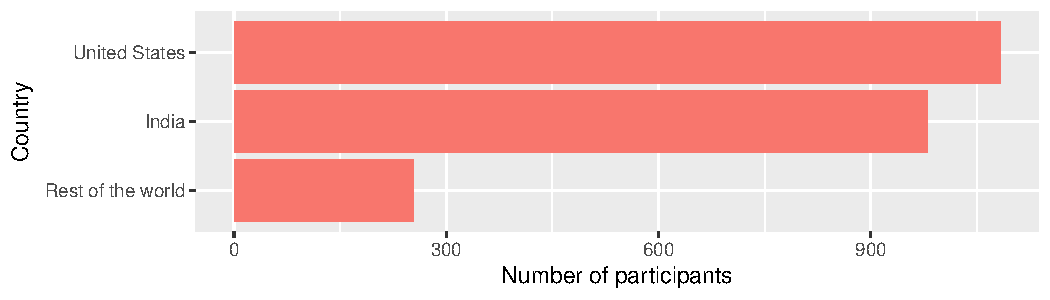
\includegraphics[width=4.5in]{turker_country.pdf} 
   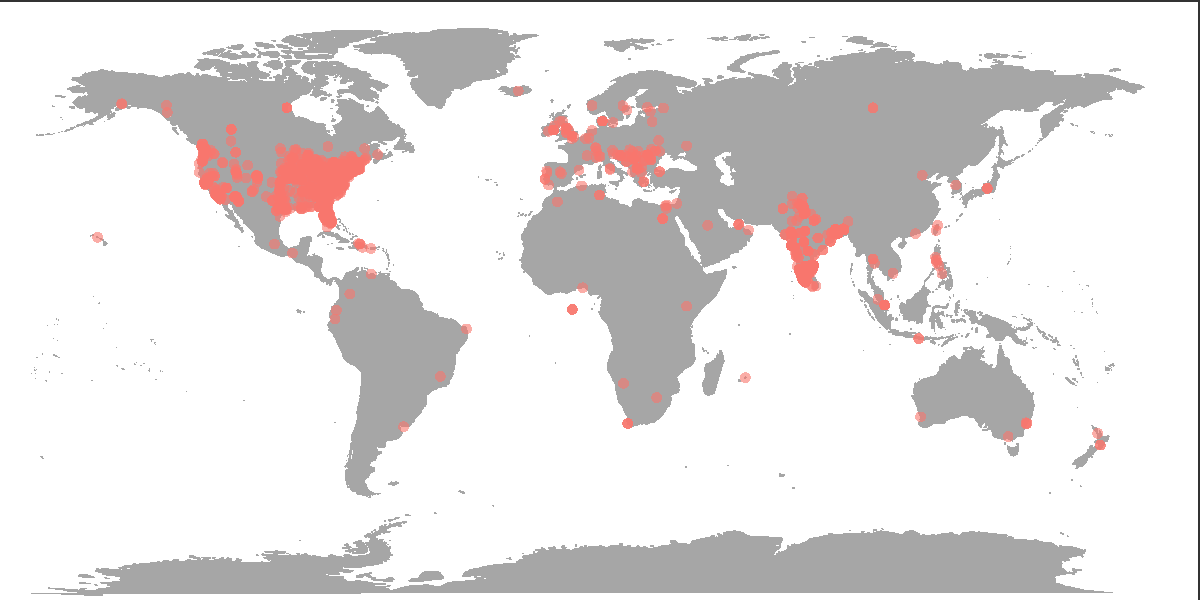
\includegraphics[width=4.5in]{turker_location.pdf}    
   \caption{Location of Amazon Mechanical Turk workers participating in the experiments. Most subjects came from India and the United States, but subjects from countries around the world took part.}
   \label{fig:turker_location}
\end{figure}

\begin{table}[hbtp]
\caption{Demographic information of the subjects participating in the MTurk experiments. Average time taken for evaluating a lineup is shown in seconds.}
\centering
\scalebox{.85}{
\begin{tabular}{rlrrcr}
  \hline
  && \multicolumn{2}{c}{Participants}&Average& Number of\\
  \cline{3-4}
 Factor & Levels & Total &\% & Time & Responses \\ 
  \hline
Gender & Female & 989 & 42.26 & 43.69 & 10538 \\ 
   & Male & 1351 & 57.74 & 48.75 & 13542 \\  
\hline
  Education & High school or less & 194 & 8.29 & 37.13 & 2253 \\ 
   & Under grad courses & 418 & 17.86 & 42.85 & 4068 \\ 
   & Under grad degree & 585 & 25.00 & 44.53 & 5792 \\ 
   & Graduate courses & 247 & 10.56 & 44.63 & 2471 \\ 
   & Graduate degree & 899 & 38.42 & 52.07 & 9496 \\ 
\hline
  Age & 18-25 & 743 & 31.75 & 43.50 & 7340 \\ 
   & 26-30 & 549 & 23.46 & 46.19 & 5610 \\ 
   & 31-35 & 375 & 16.03 & 44.19 & 3912 \\ 
   & 36-40 & 257 & 10.98 & 54.97 & 2714 \\ 
   & 41-45 & 140 & 5.98 & 43.89 & 1510 \\ 
   & 46-50 &  94 & 4.02 & 49.54 & 994 \\ 
   & above 50 & 184 & 7.86 & 52.32 & 2000 \\ 
\hline   
  Country & United States & 1086 & 46.41 & 39.65 & 10763 \\ 
   & India & 980 & 41.88 & 52.63 & 10238 \\ 
   & Rest of the world & 279 & 11.92 & 50.38 & 3079 \\ 
  
   \hline
\end{tabular}
}
\label{tbl:demographics}
\end{table}


% latex table generated in R 3.4.1 by xtable 1.8-2 package
% Wed Oct 18 17:43:02 2017
\begin{table}[ht]
\caption{\label{tbl:anova_factor}Analysis of variance (ANOVA) table comparing full model, all the demographic factors, with the reduced models, obtained by removing respective factor variable. Gender does not have a significant effect on detection rate, but does on time to respond. All factors significantly affect time to respond.}
\centering
\scalebox{0.9}{
\begin{tabular}{lrrrrlrrrr}
& \multicolumn{4}{c} {Log Time (model~\ref{eqn:demographic_time})} & &\multicolumn{4}{c} {Detection rate (model~\ref{eqn:demographic_response})}  \\
\cline{2-5} \cline{7-10} 
 & Deviance & $\chi^2$ & df & $p$-value && Deviance & $\chi^2$ & df & $p$-value \\ \cline{2-5} \cline{7-10}
Full  & 52609.1 & \multicolumn{1}{c}{---} & \multicolumn{1}{c}{---} & \multicolumn{1}{c}{---} &  & 24140.5 & \multicolumn{1}{c}{---} & \multicolumn{1}{c}{---} & \multicolumn{1}{c}{---} \\ 
 - Age & 52081.3 & 527.8 & 6 & $<$0.001 & \hspace{0.5cm} & 24113.2 & 27.3 & 6 & $<$0.001 \\ 
 - Country & 52245.5 & 363.6 & 2 & $<$0.001 &  & 24114.8 & 25.7 & 2 & $<$0.001 \\ 
 - Degree & 52498.7 & 110.4 & 4 & $<$0.001 &  & 24116.0 & 24.5 & 4 & $<$0.001 \\ 
 - Gender & 52540.3 & 68.8 & 1 & $<$0.001 &  & 24138.9 & 1.6 & 1 & 0.200 \\ 
\cline{2-5} \cline{7-10}
\end{tabular}}
\end{table}


% latex table generated in R 3.4.1 by xtable 1.8-2 package
% Wed Oct 18 23:54:25 2017
\begin{table}[hbtp]
\centering
\caption{\label{tbl:model_result_response}Parameter estimates of models \eqref{eqn:trend_response} fitted to data from three different experiments using detection rate as the response to assess learning trend. Attempt number is fitted as a factor to enable modeling any sort of non-linear learning trend. Only experiment~6 shows some evidence of a learning trend, with detection rate essentially increasing as attempts increase.}
\scalebox{.9}{
\begin{tabular}{rr>{(}r<{,}>{\hspace{-.1in}}l<{)}>{\hspace{-.15in}}l<{}cr>{(}r<{,}>{\hspace{-.1in}}l<{)}>{\hspace{-.15in}}l<{}cr>{(}r<{,}>{\hspace{-.1in}}l<{)}>{\hspace{-.15in}}l<{}}
\cline{2-5} \cline{7-10} \cline{12-15} 
& \multicolumn{4}{c} {Experiment~5} & &\multicolumn{4}{c} {Experiment~6} && \multicolumn{4}{c} {Experiment~7}\\
\cline{2-5} \cline{7-10} \cline{12-15} 
Effect & Est & 2.5\% & 97.5\% &  & \hspace{1cm} & Est & 2.5\% & 97.5\% &  & \hspace{1cm} & Est & 2.5\% & 97.5\% &  \\ 
\cline{2-5} \cline{7-10} \cline{12-15} 
Fixed \\
$\mu$ & -1.32 & -1.73 & -0.92 & *** &   & -0.16 & -0.46 & 0.13 &  &   & -1.73 & -2.81 & -0.66 & ** \\ [3pt]
  $\alpha2$ & 0.30 & -0.17 & 0.78 &  &   & 0.26 & -0.07 & 0.58 &  &   & -0.40 & -1.23 & 0.44 &  \\ 
  $\alpha3$ & -0.20 & -0.68 & 0.29 &  &   & 0.31 & -0.02 & 0.63 & . &   & -0.15 & -0.99 & 0.68 &  \\ 
  $\alpha4$ & 0.13 & -0.35 & 0.61 &  &   & 0.34 & 0.01 & 0.66 & * &   & -0.41 & -1.24 & 0.42 &  \\ 
  $\alpha5$ & 0.35 & -0.14 & 0.83 &  &   & 0.34 & 0.02 & 0.67 & * &   & -0.10 & -0.92 & 0.73 &  \\ 
  $\alpha6$ & 0.10 & -0.40 & 0.60 &  &   & 0.20 & -0.12 & 0.53 &  &   & 0.03 & -0.84 & 0.89 &  \\ 
  $\alpha7$ & 0.33 & -0.17 & 0.82 &  &   & 0.11 & -0.22 & 0.43 &  &   & -0.00 & -0.84 & 0.84 &  \\ 
  $\alpha8$ & -0.01 & -0.51 & 0.50 &  &   & 0.31 & -0.01 & 0.64 & . &   & -0.06 & -0.88 & 0.76 &  \\ 
  $\alpha9$ & -0.20 & -0.70 & 0.30 &  &   & 0.34 & 0.01 & 0.67 & * &   & 0.21 & -0.67 & 1.08 &  \\ 
  $\alpha10$ & 0.51 & 0.02 & 1.01 & * &   & 0.19 & -0.14 & 0.53 &  &   & -0.20 & -1.07 & 0.67 &  \\ 
  Random \\
  $\sigma^2_u$ & \multicolumn{5}{l}{\phantom{-}0.91}  & \multicolumn{5}{l}{\phantom{-}0.89} & 0.82   \\ 
  $\sigma^2_a$ & \multicolumn{5}{l}{\phantom{-}0.04}  & \multicolumn{5}{l}{\phantom{-}0.04} & 0.05   \\ 
  $\sigma^2_l$ & \multicolumn{5}{l}{\phantom{-}1.47}  & \multicolumn{5}{l}{\phantom{-}1.43} & 3.38   \\ \cline{2-5} \cline{7-10} \cline{12-15} 
\\
\hline
\multicolumn{10}{l}{Signif. codes:  *** $<$ 0.001 $\le$ ** $<$ 0.01 $\le$ * $<$ 0.05 $\le$ . $<$ 0.1 $\le$ ` ' $<$ 1}
\end{tabular}}
\end{table}


% latex table generated in R 3.4.1 by xtable 1.8-2 package
% Wed Oct 18 23:37:55 2017
\begin{table}[bhtp]
\caption{\label{tbl:model_result_time}Parameter estimates of model~\eqref{eqn:trend_time} fitted for log time taken to evaluate a lineup. Both fixed effects parameters of Attempt ($\alpha_1$ and $\alpha$) are highly significant for all three experiments~5,~6 and~7.}
\centering
\scalebox{0.9}{
\begin{tabular}{lr>{(}r<{,}>{\hspace{-.1in}}l<{)}>{\hspace{-.15in}}l<{}cr>{( }r<{,}>{\hspace{-.1in}}l<{)}>{\hspace{-.15in}}l<{}cr>{(}r<{,}>{\hspace{-.1in}}l<{)}>{\hspace{-.15in}}l<{}}
\cline{2-5} \cline{7-10} \cline{12-15} 
& \multicolumn{4}{c} {Experiment~5} & &\multicolumn{4}{c} {Experiment~6} && \multicolumn{4}{c} {Experiment~7}\\

\cline{2-5} \cline{7-10} \cline{12-15} 
\multicolumn{2}{c}{Effect \hfill Est} & 2.5\% & 97.5\% &  &  & Est & 2.5\% & 97.5\% & &  & Est & 2.5\% & 97.5\% & \\ 
  \cline{2-5} \cline{7-10} \cline{12-15}
\multicolumn{2}{l}{Fixed}\\
$\mu$ & 3.80 & 3.72 & 3.88 & *** &   & 3.89 & 3.83 & 3.96 & *** &   & 3.75 & 3.64 & 3.85 & *** \\ 
  $\alpha_1$ & 0.32 & 0.25 & 0.39 & *** &   & 0.34 & 0.28 & 0.40 & *** &   & 0.28 & 0.18 & 0.38 & *** \\ 
  $\alpha$ & -0.04 & -0.05 & -0.03 & *** &   & -0.04 & -0.05 & -0.03 & *** &   & -0.03 & -0.04 & -0.02 & *** \\ 
\multicolumn{2}{l}{Random}\\
  $\sigma^2_u$ & \multicolumn{5}{l}{\phantom{-}0.52}   & \multicolumn{5}{l}{\phantom{-}0.49}  & 0.37   \\ 
  $\sigma^2_a$ & \multicolumn{5}{l}{\phantom{-}0.03}  & \multicolumn{5}{l}{\phantom{-}0.05}   & 0.05   \\ 
  $\sigma^2_l$ & \multicolumn{5}{l}{\phantom{-}0.09}   & \multicolumn{5}{l}{\phantom{-}0.20}   & 0.24   \\
  $\sigma^2$ & \multicolumn{5}{l}{\phantom{-}0.46}   & \multicolumn{5}{l}{\phantom{-}0.50}  & 0.45  \\ 
   \cline{2-5} \cline{7-10} \cline{12-15}
\end{tabular}}
\end{table}




\begin{table*}[hbtp] 
\centering 
\caption{Overview of 10 different Turk experiments, from which data was collected to study human factor effects. All of the experimental data were used to estimate the effect of demographic factors (DF) on visual inference while three were suitable for assessing learning trend (LT) and location effect (LE) was possible to assess using just one specially designed study.} 
\begin{tabular}{m{.5cm}m{2.6cm}m{2cm}m{5.5cm}m{3cm}} 
\hline\hline 
 & Experiment &  Test Statistic  & Lineup question & Used in study of\\ [0.5ex] % inserts table %heading 
\hline 
1  & Box plot & \begin{minipage}[t]{2cm} \begin{center}	\scalebox{0.12}{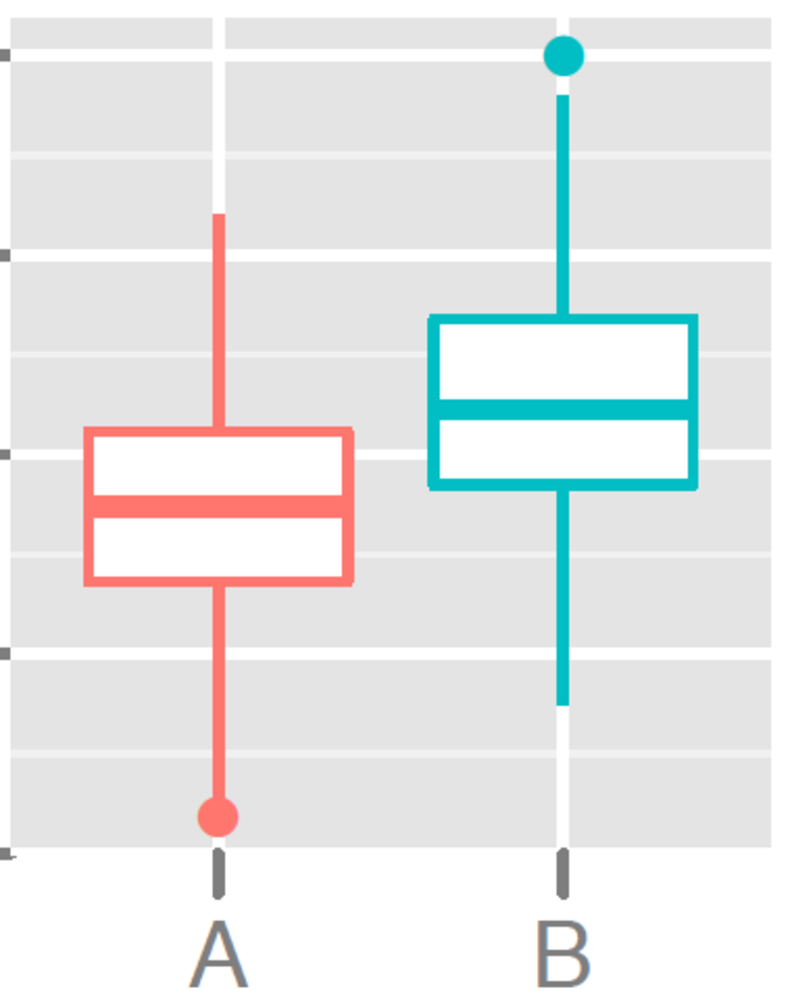
\includegraphics{stat_category1.pdf}} \end{center} \end{minipage} & Which set of box plots shows biggest vertical difference 
between group A and B? & DF\\
2 &  Scatter plot & \begin{minipage}[t]{2cm}  \begin{center} \scalebox{0.3}{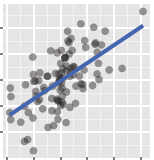
\includegraphics{stat_beta_k1.png}} \end{center} \end{minipage} & Of the scatter plots below which one shows data that has steepest slope? & DF\\
  3 & Contaminated plot &\begin{minipage}[t]{2cm} \begin{center} \scalebox{0.5}{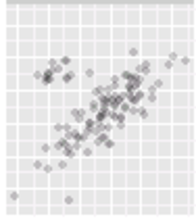
\includegraphics{stat_contaminated.pdf}} \end{center} \end{minipage} & Of the scatter plots below which one shows data that has steepest slope? & DF\\
 4 & Polar vs Cartesian & \begin{minipage}[t]{2cm} \begin{center}  \scalebox{0.32}{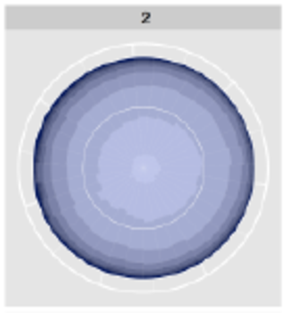
\includegraphics{stat_polar.pdf}} \end{center} \end{minipage} &Which plot is different?& DF\\
  5 & Hist vs density & \begin{minipage}[t]{2cm} \begin{center}  \scalebox{0.38}{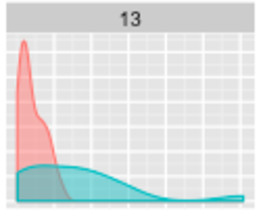
\includegraphics{stat_density.pdf}} \end{center} \end{minipage} &In which plot is the blue group furthest to the right?&  DF \hfill LT \hfill \phantom{.} \hfill \phantom{.} \\  
  6 & Violin vs boxplot & \begin{minipage}[t]{2cm} \begin{center}  \scalebox{0.35}{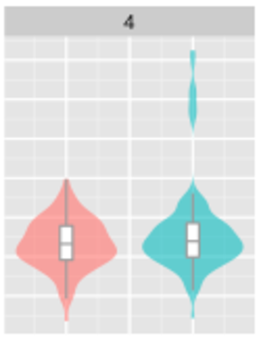
\includegraphics{stat_violin.pdf}} \end{center} \end{minipage}&  In which plot does the blue group look the most different from  the red group? &  DF  \hfill LT \hfill \phantom{.} \hfill \phantom{.} \\
  7 & Group separation & \begin{minipage}[t]{2cm} \begin{center}  \scalebox{0.4}{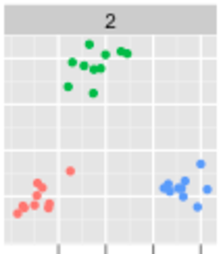
\includegraphics{stat_separation.pdf}} \end{center} \end{minipage} &Which of these plots has the most separation between the coloured groups? & DF  \hfill LT \hfill \phantom{.} \hfill \phantom{.} \\ 
  8 & Sine Illusion & \begin{minipage}[t]{2cm} \begin{center}  \scalebox{0.28}{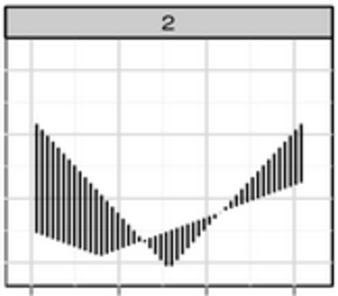
\includegraphics{stat_sine.pdf}} \end{center} \end{minipage} & In what picture is the size of the curve most consistent? & DF\\ 
  9 & Gene expression &\begin{minipage}[t]{2cm} \begin{center}  \scalebox{0.45}{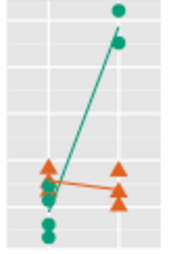
\includegraphics{stat_gene.pdf}} \end{center} \end{minipage} & In which of these plots is the green line the steepest, and the spread of the green points relatively small? & DF  \hfill \phantom{LT} \hfill {LE} \hfill \phantom{.}\\ 
  10 & Test normality & \begin{minipage}[t]{2cm} \begin{center}  \scalebox{0.35}{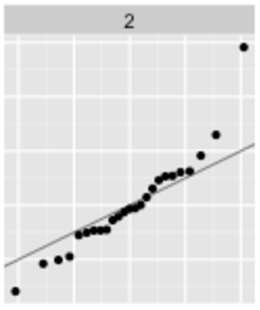
\includegraphics{stat_normality.pdf}} \end{center} \end{minipage} &Which of these plots is most different from the others? & DF\\ 

\hline 
\end{tabular} 
\label{tbl:visual_stat} 
\end{table*} 


\end{document}


